\documentclass[11pt,french,a4paper]{report}
\usepackage[utf8]{inputenc}
\usepackage[left=2cm,right=2cm,top=2cm,bottom=2cm]{geometry}
\geometry{a4paper} 
\usepackage{graphicx} %Inclure images 
\usepackage{listings} %Style code C 
\usepackage[french]{babel} %Document en FR
\frenchbsetup{StandardLists=true}
\usepackage[T1]{fontenc}
\usepackage{enumitem}
\usepackage{pifont}
\usepackage{lastpage}
\usepackage{fancyhdr}
\pagestyle{fancy}
\usepackage{pdfpages}
\usepackage[pdftex]{graphicx}
\usepackage{eurosym}

\fancyhead[L]{\includegraphics[scale=00.3]{../../logo/logo_um.PNG}
\includegraphics[scale=0.06]{../../logo/logo_lirmm.png}}
\fancyhead[C]{Rapport de Présentation - LIRMM - SuperBeeLive}
\fancyhead[R]{\includegraphics[scale=0.03]{../../logo/logo_polytech.png} \includegraphics[scale=0.3]{../../logo/logo_se.jpg}}
\fancyfoot[L]{\small Olivia SERENELLI-PESIN\normalsize}
\fancyfoot[C]{\includegraphics[scale=0.04]{../../logo/logo_superbeelive.png}}
\fancyfoot[R]{\thepage/\pageref{LastPage}}
\renewcommand{\footrulewidth}{0pt}
\renewcommand{\headrulewidth}{0.4pt}


\makeatletter
\let\ps@plain=\ps@fancy
\makeatother

\begin{document}

    \title{
        \includegraphics[width=2cm]{../../logo/logo_um.PNG}\hspace{5cm} 
           
\includegraphics[width=5cm]{../../logo/logo_lirmm.png} \\
           \normalsize\textsc{}
           \hfill \\
           }
         
    \author{
        \LARGE{\textbf{Rapport d'entreprise du Semestre 5}} \\\\ 
        \LARGE{\textbf{LIRMM}} \\
           \large{\textbf{Laboratoire d'Informatique, de Robotique et de Microélectronique de Montpellier}} \\ \\
           \large{\textbf{161 Rue Ada, 34095 Montpellier}} \\
           \large{\textbf{SIRET : 130 020 548 00017}} \\ \\
           \large{Apprentie : \textbf{Olivia SERENELLI-PESIN}} \\
           \large{Maître d'apprentissage : \textbf{Sébastien DRUON}} \\
           \large{Tutrice accadémique : \textbf{Karen GAUDARY-JEAN}} \\ \\
           \large{SE3 - Promotion 2019-2022} \vspace*{5\baselineskip}
            \bigskip \\
            \includegraphics[width=5cm]{../../logo/logo_polytech.png}\hspace{7cm}
            \includegraphics[width=2cm]{../../logo/logo_se.jpg}
            \date{}
            }
\maketitle

\clearpage
\newpage 

\tableofcontents

\chapter{Présentation de l'entreprise}

\section{L'entreprise : le LIRMM}

Mon apprentissage en Système Embarqué s'inscrit dans un contexte de Recherche. Embauchée par l'Université 
de Montpellier, je travaille au LIRMM (Laboratoire d'Informatique, de Robotique et de Microélectronique de Montpellier) 
au sein de l'équipe EXPLORE, spécialisée dans la conception de robot pour l'exploration sous marine. \\
Plus précisement, j'ai été affectée au projet SuperBeeLive en tant qu'ingénieure de recherche afin de seconder M. Druon, 
mon maître d'apprentissage, dans les diverses tâches qu'il est amené à réaliser dans ce projet. \\

Le LIRMM est une Unité Mixte de Recherche situé au Campus Saint-Priest qui dépend du Centre Nationnal de Recherche Scientifique, de l'Université de Montpellier
et de l'Institut National de Recherche en Informatique et en Automatique. 
Ainsi, on retrouve plusieurs types d'employés : des enseignants chercheurs qui dépendent de l'UM, des chercheurs qui dépendent du CNRS
ou de l'INRIA, du personnel technique de soutien (ingénieurs et techniciens) qui peuvent dépendre de l'une des trois composantes et 
d'étudiants. En effet, l'un des rôles principal des enseignants chercheurs est de diffuser la connaissance, ils sont donc très souvent 
impliqués dans des stages en laboratoire. 

Le laboratoire est constitué de trois départements scientifiques : 
\begin{itemize}
    \item Informatique
    \item Microélectronique
    \item Robotique
\end{itemize} 
Le département informatique s'étend des mathématiques à la recherche appliquée : algorithmique des graphes, bioinformatique,
cryptographie, réseaux, base de données et système d'information, génie logiciel, intelligence artificielle, interaction homme-machine.
Le département microélectronique s'interesse aux domaines de la conception et du test de systèmes intégrés et microsystèmes.
Enfin, le département Robotique va s'intéreseer aux problématiques de synthèse, de supervision et de gestion des systèmes dynamiques
complexes et de navigation, localisation et de pilotage de véhicules autonomes présents ou distants. 

\section{L'équipe EXPLORE}
L'équipe EXPLORE fait parti du département Robotique depuis 2012 suite à une restructuration interne.
Historiquement, le centre d'intérêt principal de l'équipe est la conception et le développement des outils 
théoriques et expérimentaux de la robotique mobile pour l'exploration intégrée de l'environnement.
Aujourd'hui les travaux de l'équipe se focalisent sur les problématiques scientifiques relevant de 
la robotique sous-marine. A terme, le but d'EXPLORE est de pouvoir indiquer si nous sommes capables de 
développer des systèmes robotiques sous-marins pouvant réaliser en confiance et en autinomie des missions
complexes malgré la sévérité des contraintes imposées par le milieu aquatique. 
Afin de pouvoir répondre à cette question, l'équipe EXPLORE mobilise les compétences complémentaires de ses membres, 
allant du contole du mouvement, à la perception, la cartographie centrée modèle perception/action, aux architectures 
de contrôle et de la sûreté de fonctionnement. 
Ces compétences sont apportées par une équipe de 7 permanents Professeurs des Universités et Maître de Conférences, 2 Ingénieurs Techniciens 
et Enseignant Chercheur et 5 doctorants. 

Nous pouvons citer 4 projets majeurs pilotés par EXPLORE de 2016 à 2022. 
\begin{itemize}
    \item ALEYIN : projet étandard du labex NUMEV (2016-2019) - Exploration des galeries karstiques - $300k$\euro{}
    \item REEA : agglomération de Béziers (2016-2019) - Génération de trajectoires pour l'observation de cibles mobiles - $60k$\euro{} 
    \item DEDAL : projet industriel avec Naval Group (2018-2019) - Génération de trajectoires pour l'observation de cibles mobiles - $32k$\euro{} 
    \item BUBOT : projet I-site MUSE (2019-2022) - Outils pour l'observation et l'étude de la biodiversité marine - $125k$\euro{} 
\end{itemize}

En plus de ces projets majeurs, l'équipe est partenaire d'autres projets de recherches, comme SuperBeeLive avec comme responsable 
de projet dans l'équipe M. Druon et comme participants principaux, M. Triboulet et moi même. Le montant de ce projet 
s'élève à $96k$\euro{}.

Ainsi, l'équipe est concentrée sur des recherches pour des robots dans les milieux sous-marins, mais il n'empêche pas d'y voir
des collaborations avec d'autres équipes et laboratoire sur des projets plus terrestres. 

La conception de robots marins et subaquatique va de paire avec les projets de l'équipe, ainsi nous retrouvons plusieurs robots
construit ou en cours de constructions :
\begin{itemize}
    \item ULYSSE a été conçu pour réaliser les premières expérimentations en milieu karstique et a servi de 
        base à l'étude algébrique des propriétés du sous-système d'actionnement.
    \item REMI a été conçu en partenariat avec les entreprises Syera et Reeds pour participer à des
        campagnes expérimentales d'études de la biodiversité marine en collaboration avec les 
        biologistes de MARBEC.
    \item TELEMATIQUE est en cours de fabrication. Il prend le relais d'Ulusse pour les
        futures explorations karstiques. 
    \item CUNE est un robot sur-actionné permettant la validation des lois de commande et des 
        algorithmes d'optimisation de l'acionnement.
    \item SENTINELLE est un système redondant à géométrie d'actionnement variable et commandable. Il permet de
        valider les algorithmes de commande et d'optimisation d'actionnement. 
    \item UWRS est un syst-me bio-inspiré de l'anguille permettant de produire une propulsion par 
        déformation du corps. Son objectif est de valider l'approche de la gestion de la redondace à la locomotion.
    \item BAVION est un système de surface conçu en collaboration avec l'évole Polytech Montpellier qui préfigure les développements 
        réalisés par NEOCEAN et le projet ASV.
\end{itemize} 

Voici quelques robots qui ont été crées par l'équipe EXPLORE

\begin{figure}[!h]
    \centering 
    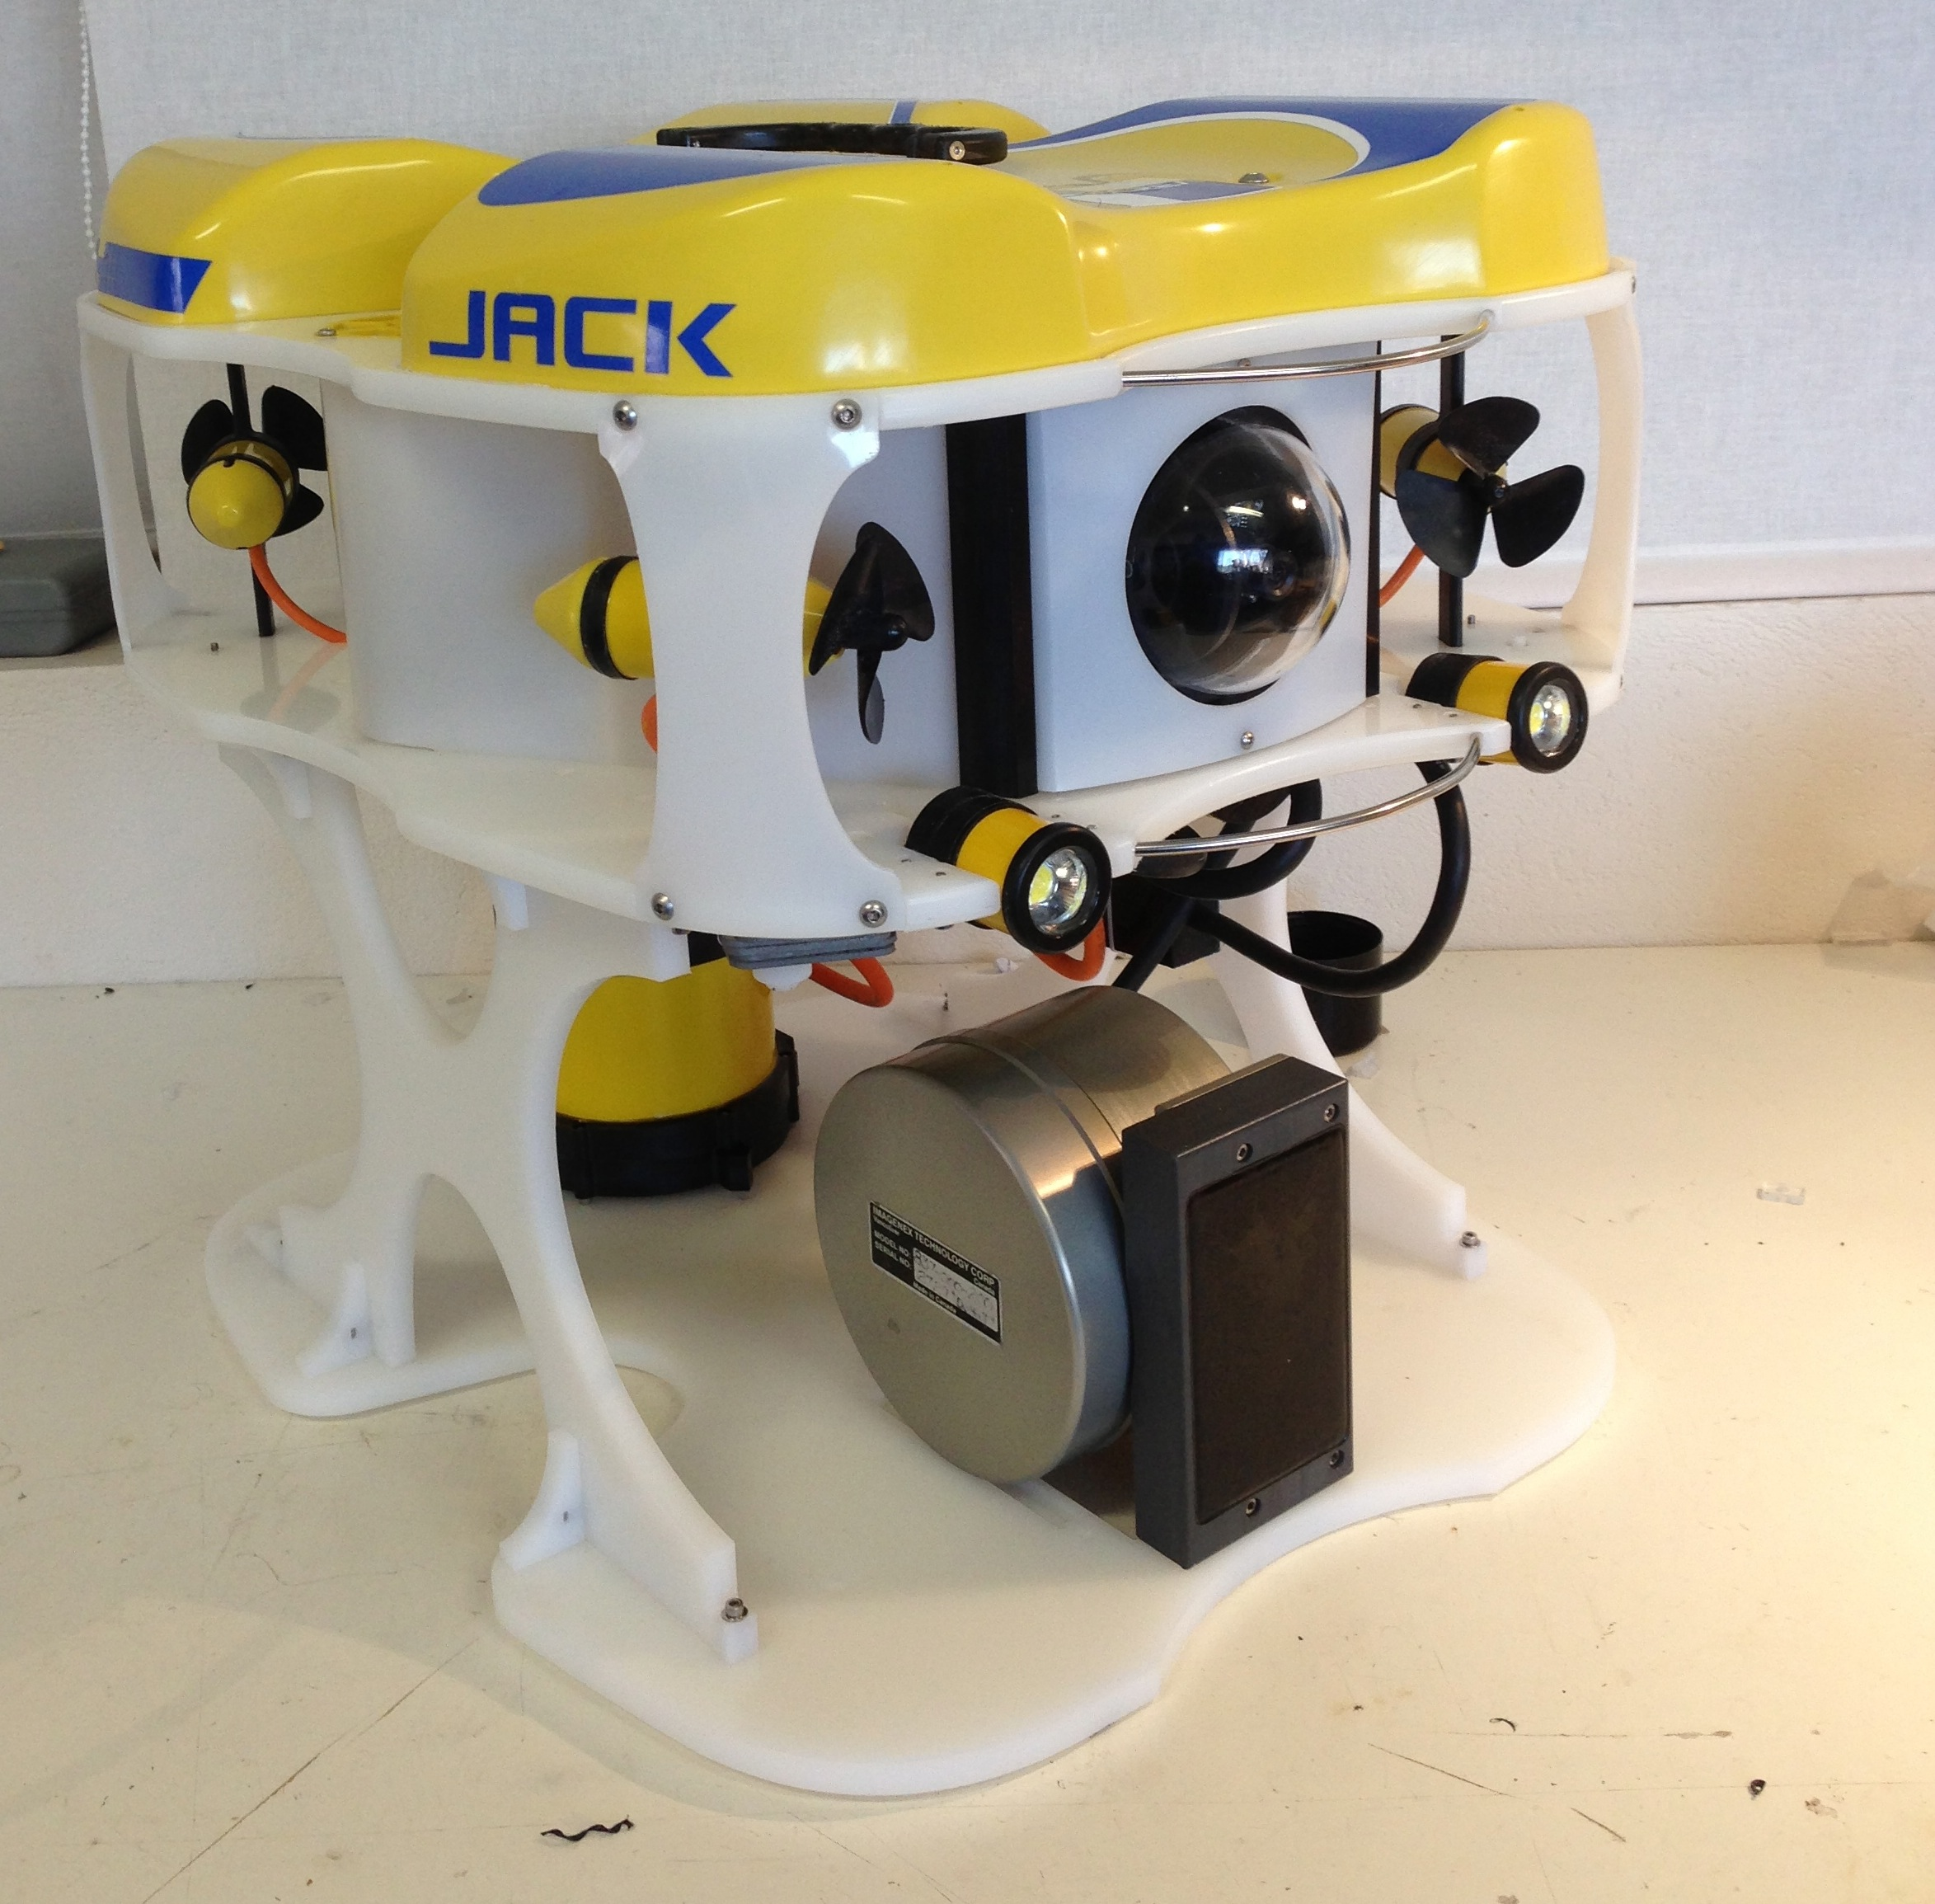
\includegraphics[width=5cm]{./img/robot_jack.jpg}
    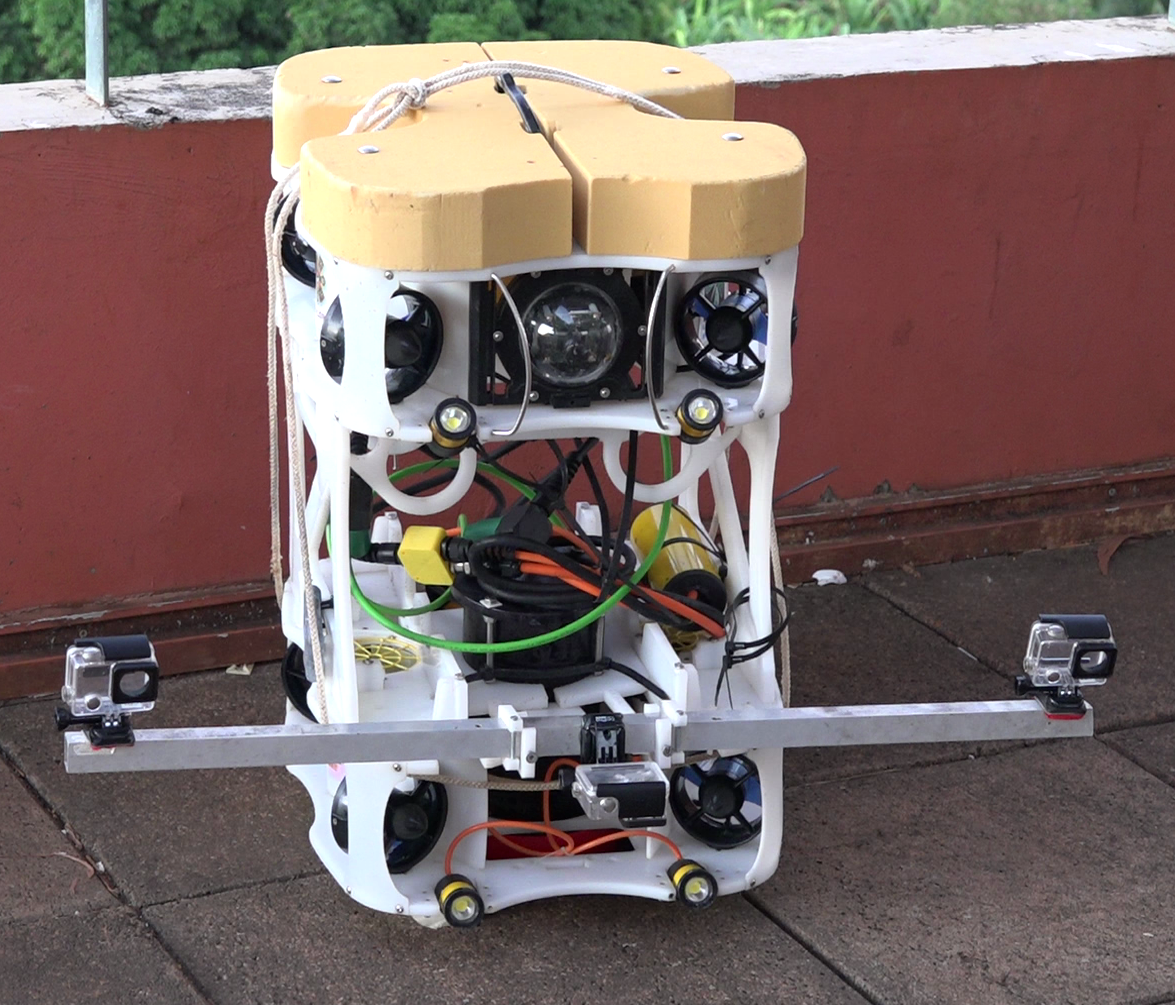
\includegraphics[width=5cm]{./img/robot_ulysse.png}
    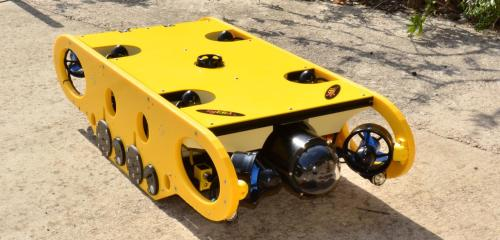
\includegraphics[width=5cm]{./img/robot.jpg}
    \caption{Robots de l'équipe Superbeelive, dans l'ordre : Jack, Ulysse et Rémi}
    \label{robot}
\end{figure}

\clearpage

\section{Le projet SuperBeeLive}

La santé et le développement des abeilles sont aujourd’hui des questions de plus en plus étudiées. Les bouleversements
majeurs de notre planète et de l’activité humaine se traduisant par une augmentation alarmante de la mortalité
des colonies et une chute de la production du miel dans nos pays développés, il est urgent de se préoccuper de leur futur. 
La situation des abeilles domestiques alerte le pouvoir public sur l’accélération de la dégradation de la biodiversité des 
pollinisateurs domestiques et sauvages, et de la flore qui en dépend. Ces dégâts sont dûs, entre autres, à l’apparition 
et la prolifération d’espèces invasives pour les abeilles, provoquant maladies et détériorations. \\ 
Le projet consiste en la structuration de plusieurs collaborations existantes ou nouvelles autour du développement 
d’une ruche plate instrumentée destinée au monitorage détaillé de la santé de l’abeille et des écosystèmes. Son but est de
pouvoir répondre à des questions clé, notamment autour des mécanismes physiopathologiques et des maladies chroniques 
dûes aux parasites ainsi qu’aux altérations de l’écosystèmes et des qualités nutritives des produits des ruches. \\
Répondre à ces questions permettra de regrouper différentes solutions technologiques systèmatiques, 
automatiques et non-invasives à la collection de données usuelles déterminantes dans chacun des thèmes abordés.
Les différents travaux déjà effectués autour de ce sujet ne visaient qu’un seul type de problème à la fois, 
ne permettant pas une vision globale des difficultés rencontrées par les abeilles. Notre but est de réunir les différentes
données qui peuvent être utilisés pour étudier l’influence des éléments et événements extérieurs sur leur santé et leur cadre de vie.\\

Concrètement, l'équipe de SuperBeeLive va concevoir une ruche plate \footnote{Voir figures \ref{images_ruche_plate}} afin d'y mettre 
en place plusieurs type  de capteurs (hygrométrie, vibrations, température interne et externe, etc) ainsi que des caméras qui filmeront.
\begin{figure}[!h]
    \centering 
    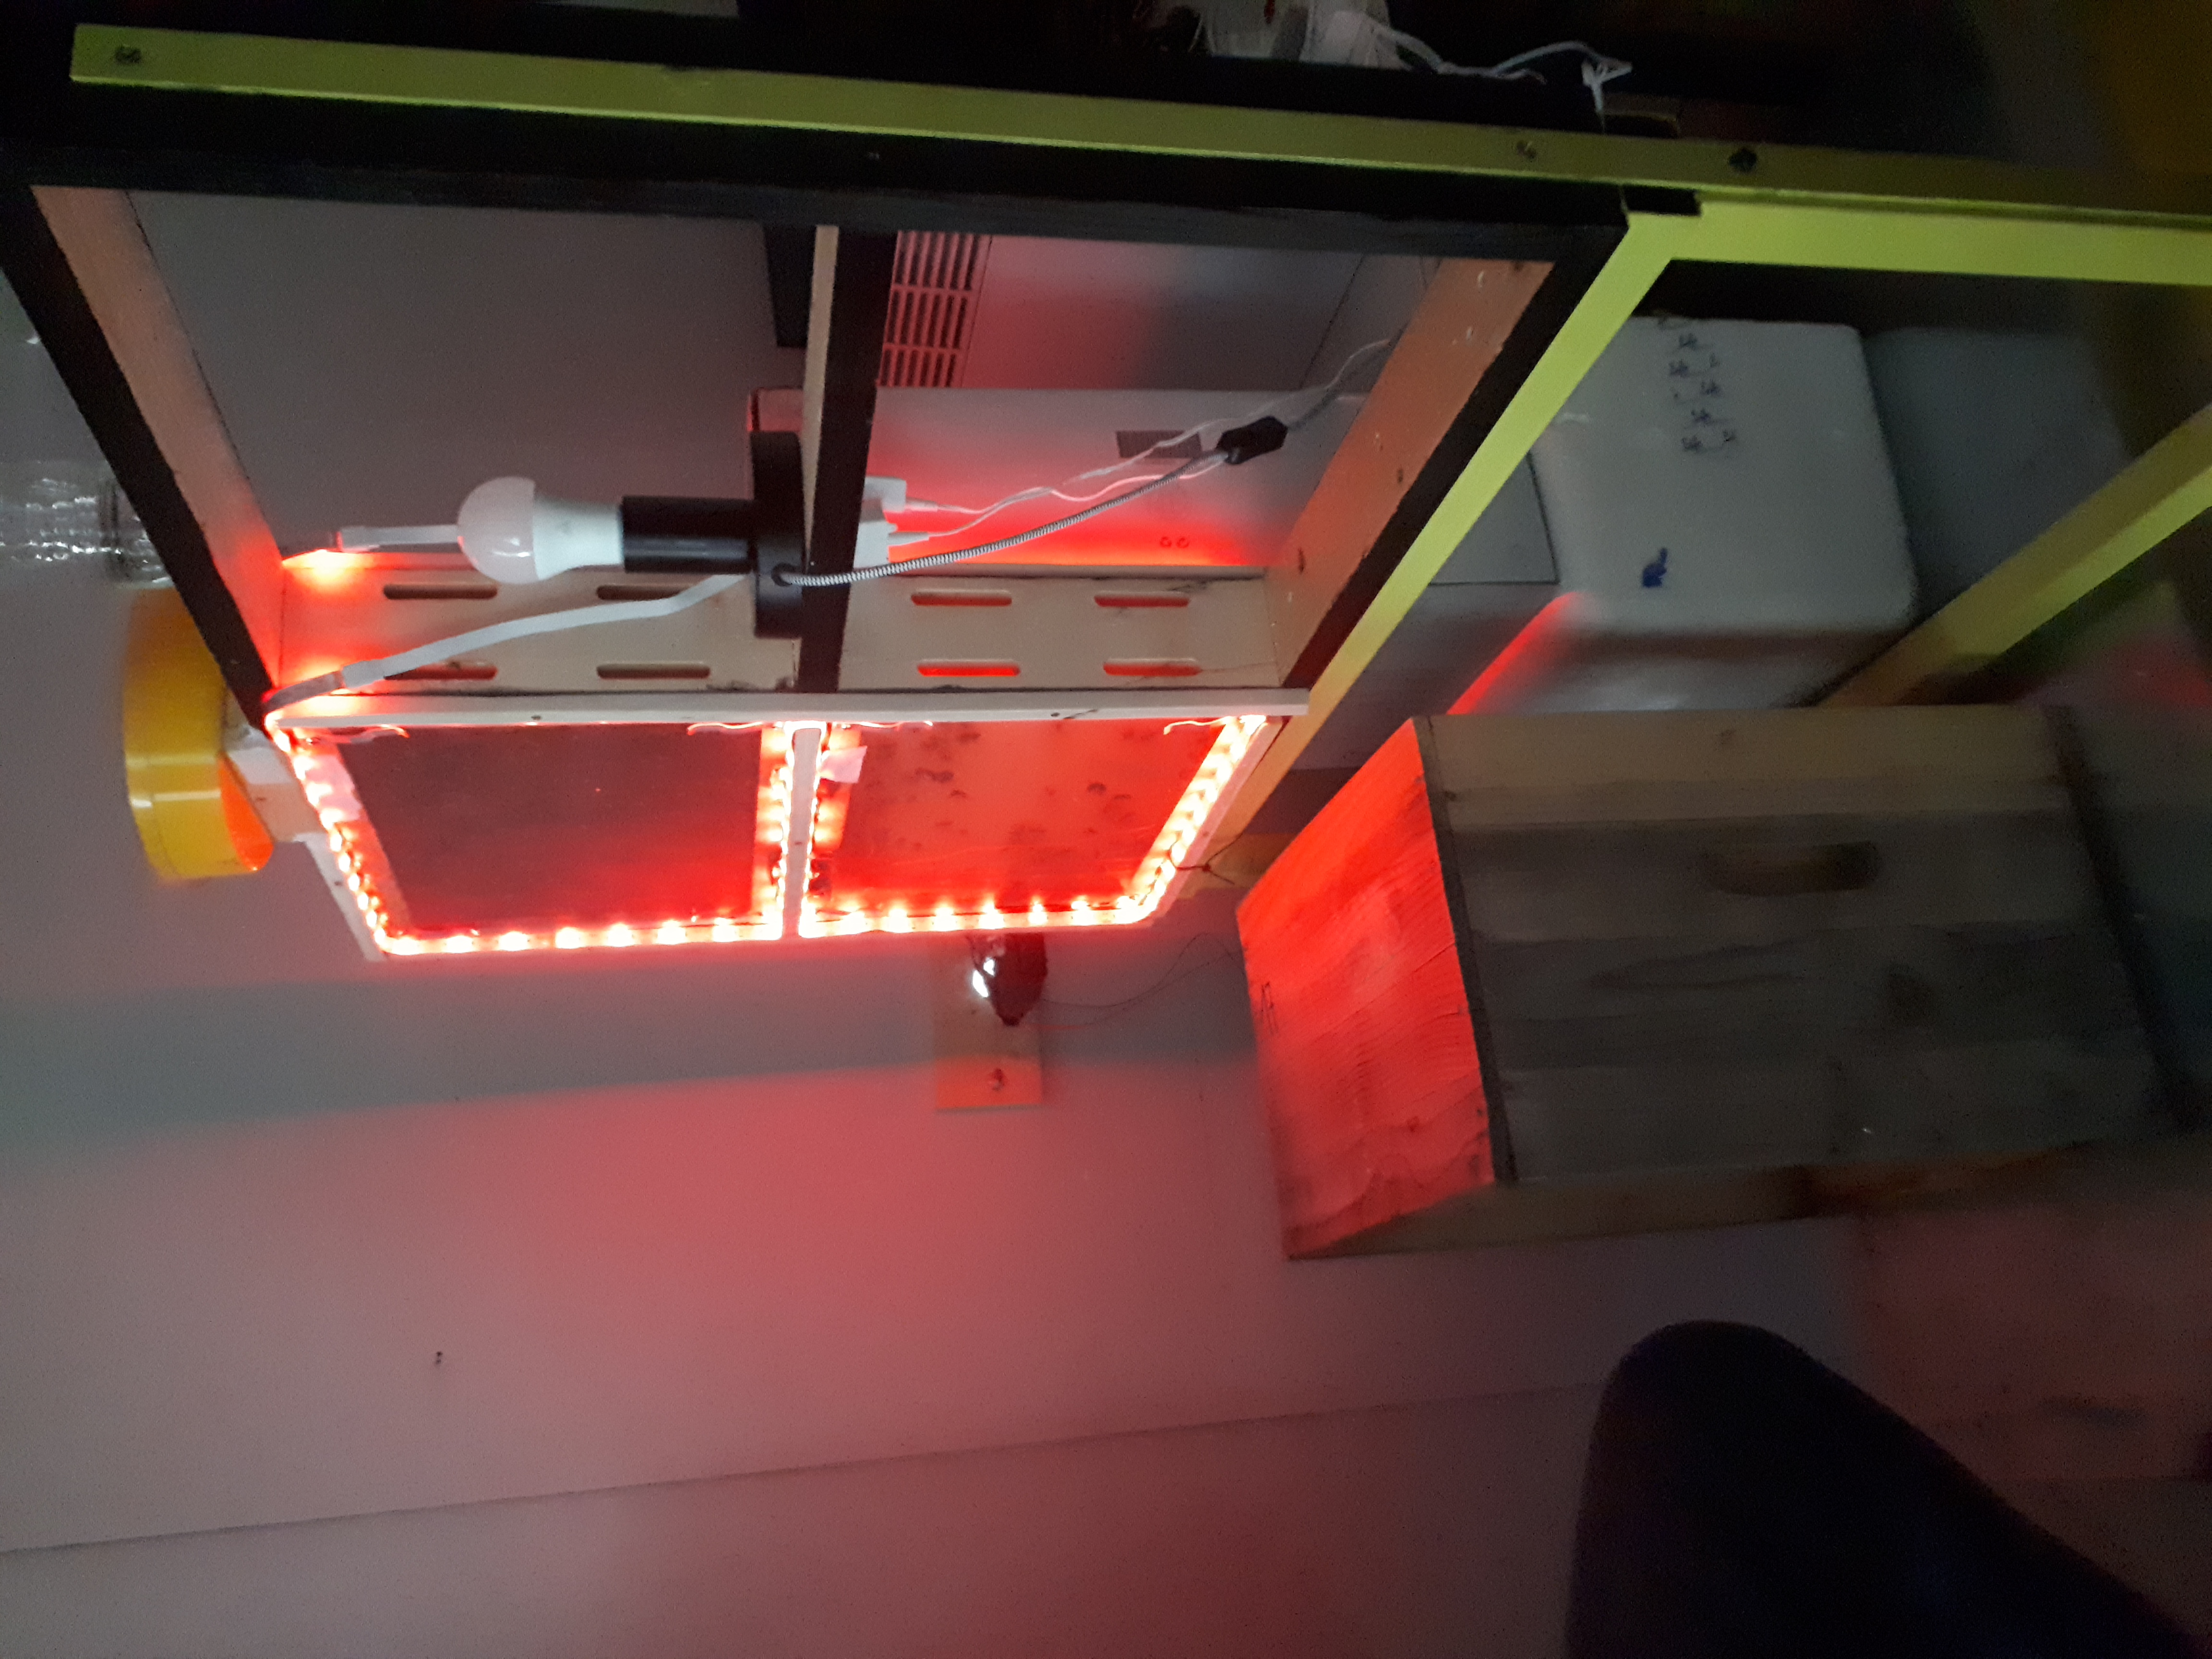
\includegraphics[width=5cm,angle=270]{./img/cote_ruche.jpg} 
    \includegraphics[width=5cm,angle=270]{./img/face_ruche.jpg} \\
    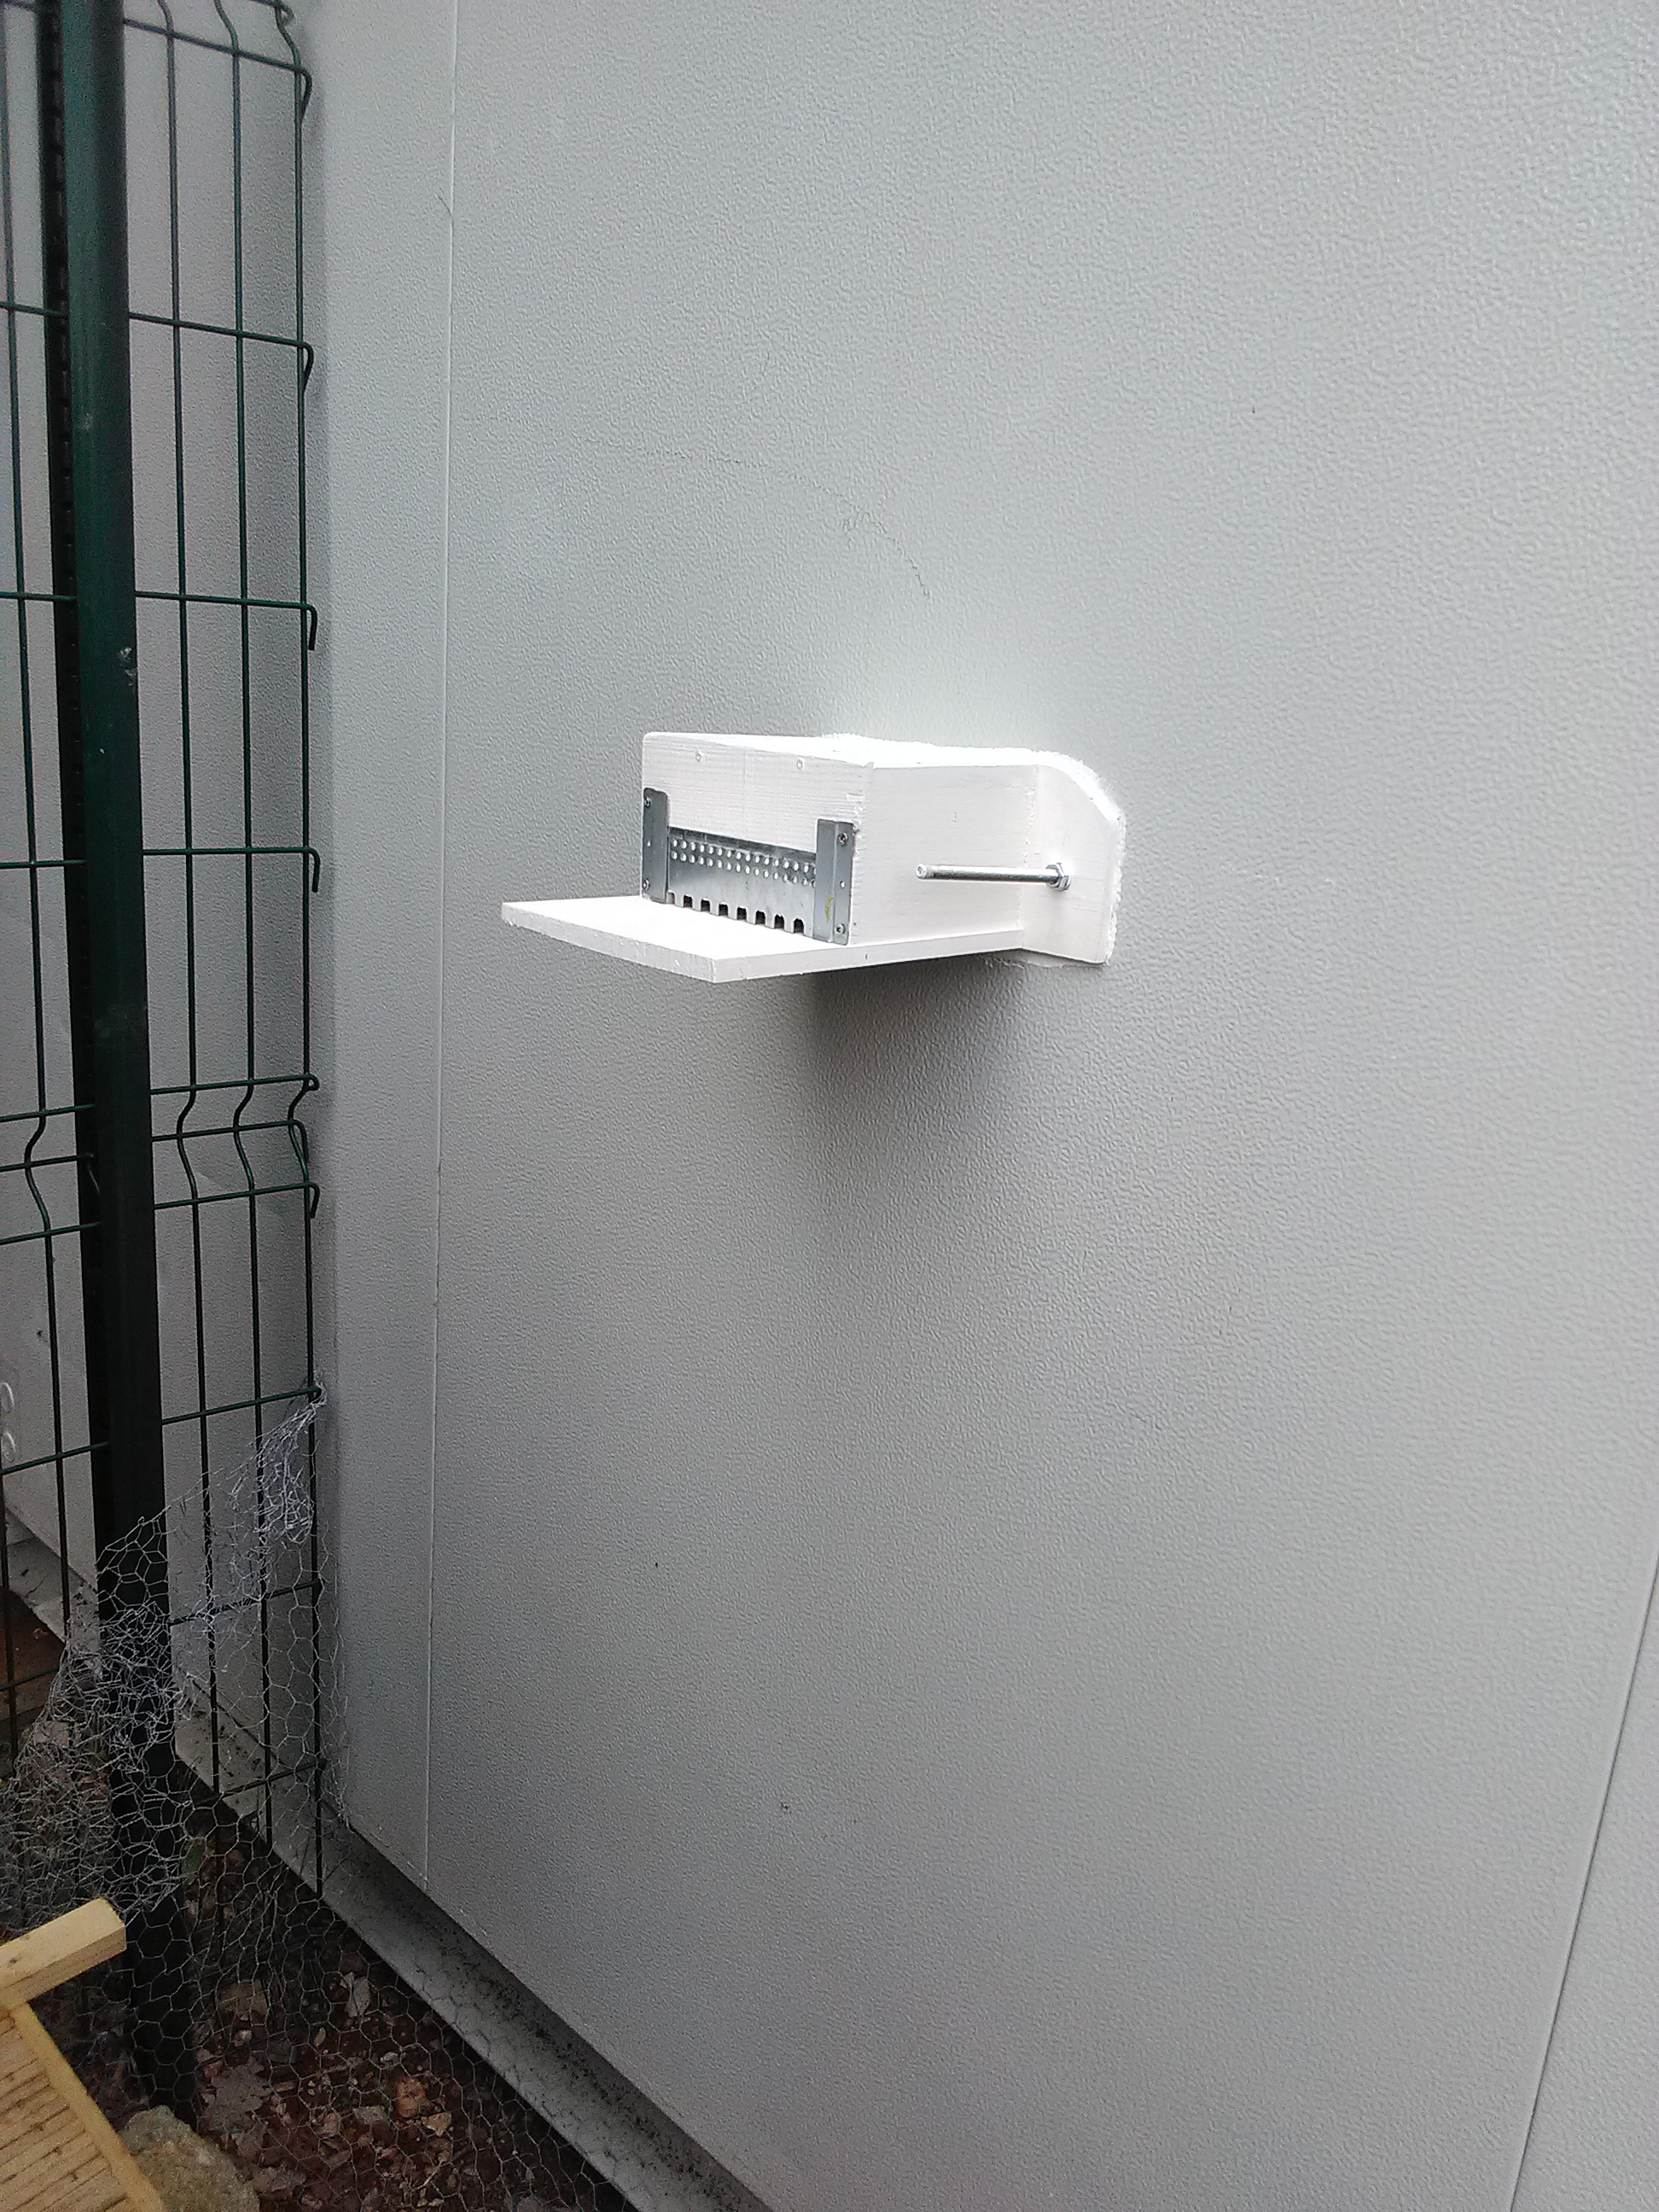
\includegraphics[width=3cm]{./img/photo_exterieur_ruche.jpg}
    \caption{Photos de la ruches plate}
    \label{images_ruche_plate}
\end{figure}

Dans un premier temps, cette instrumentation nous permettra d'observer en temps réel la ruche et ses habitantes : 
les caméras nous donnerons une vision globale de ce qu'il s'y passe, aussi bien en intérieur pour observer leur 
comportement et tenter de repérer des parasites comme le varoa \footnote{Voir bibliographie \cite{site5}}, 
qu'en extérieur pour y voir les dangers comme le frelon asiatique \footnote{Voir bibliographie \cite{site6}}.
Couplée aux donnés récoltées à l'aide de la carte électronique et ses capteurs installés au centre de la ruche plate, 
nous pourrons avoir une vision complète et détaillée des événements et leur répercutions ponctuant la vie d'une colonie,
de sa naissance à sa mort. \\
Ces observations ont pour but d'être enregistrée, sauvegardées et commentées par les biologistes afin de construire une base
de donnée contenant plusieurs types de comportements reconnus comme le refroidissement de la ruche, les danses frétillante \footnote{Voir bibliographie \cite{ref10}}, 
etc.  
\\
Dans un second temps, cette base de donnée pourra être utilisée afin de créer des algorithmes repérant ces différents comportements
de manière automatisée. Cela nous permettrait, en plus d'avoir des données complètes, d'en avoir leur analyse en 
temps réel. Ces informations seront diffusées de deux façons. D'abord, elles seront partagées pour être étudiées par d'autres scientifiques, 
notamment les collaborateurs du projet SuperBeeLive. Le projet se veut aussi éducatif : une vitrine Web accessible au public 
sera créée présentant une ruche, ses données numériques et les vidéos commentées en direct par les algorithmes. \\


Ainsi, les ruches plates de SuperBeeLive permettront de fournir des données cruciales pour des futures recherches sur les 
abeilles. En plus, elles informeront le grand public sur leur importance et aux risques liées à nos activités humaines pour 
cette espèce et la biodiversité. 


\subsection{L'équipe Superbeelive}
Le projet étant dans le domaine de la biologie, celui-ci est réalisé par plusieurs laboratoires de recherches. 
Les deux laboratoires porteurs du projets sont l'IBMM, L'institut des Biomolécules Max Mousseron avec Matthieu Rousset
et le CNRS, Centre National de la Recherche Scientifique avec Jean-Baptiste THIBAUD. On y retrouve également le LMGC, Laboratoire
de Mécanique et Génie Civil où sont réalisés les prototypes de la ruche plate et le LIRMM. 
En plus des laboratoires de recherches, une composante étudiante participe aussi au projet : l'IUT de Béziers, avec comme représentant
Philipe PUJAS, qui mettent à contribution les étudiants via des projets. Enfin, des partenaires internationnaux participent également :
l'Université de Wageningen. 
Le schéma suivant représente l'organigramme du projet avec le noms des personnes avec qui je travaille. \footnote{Voir figure \ref{orga_sbl}}

\begin{figure}[!h]
    \centering 
    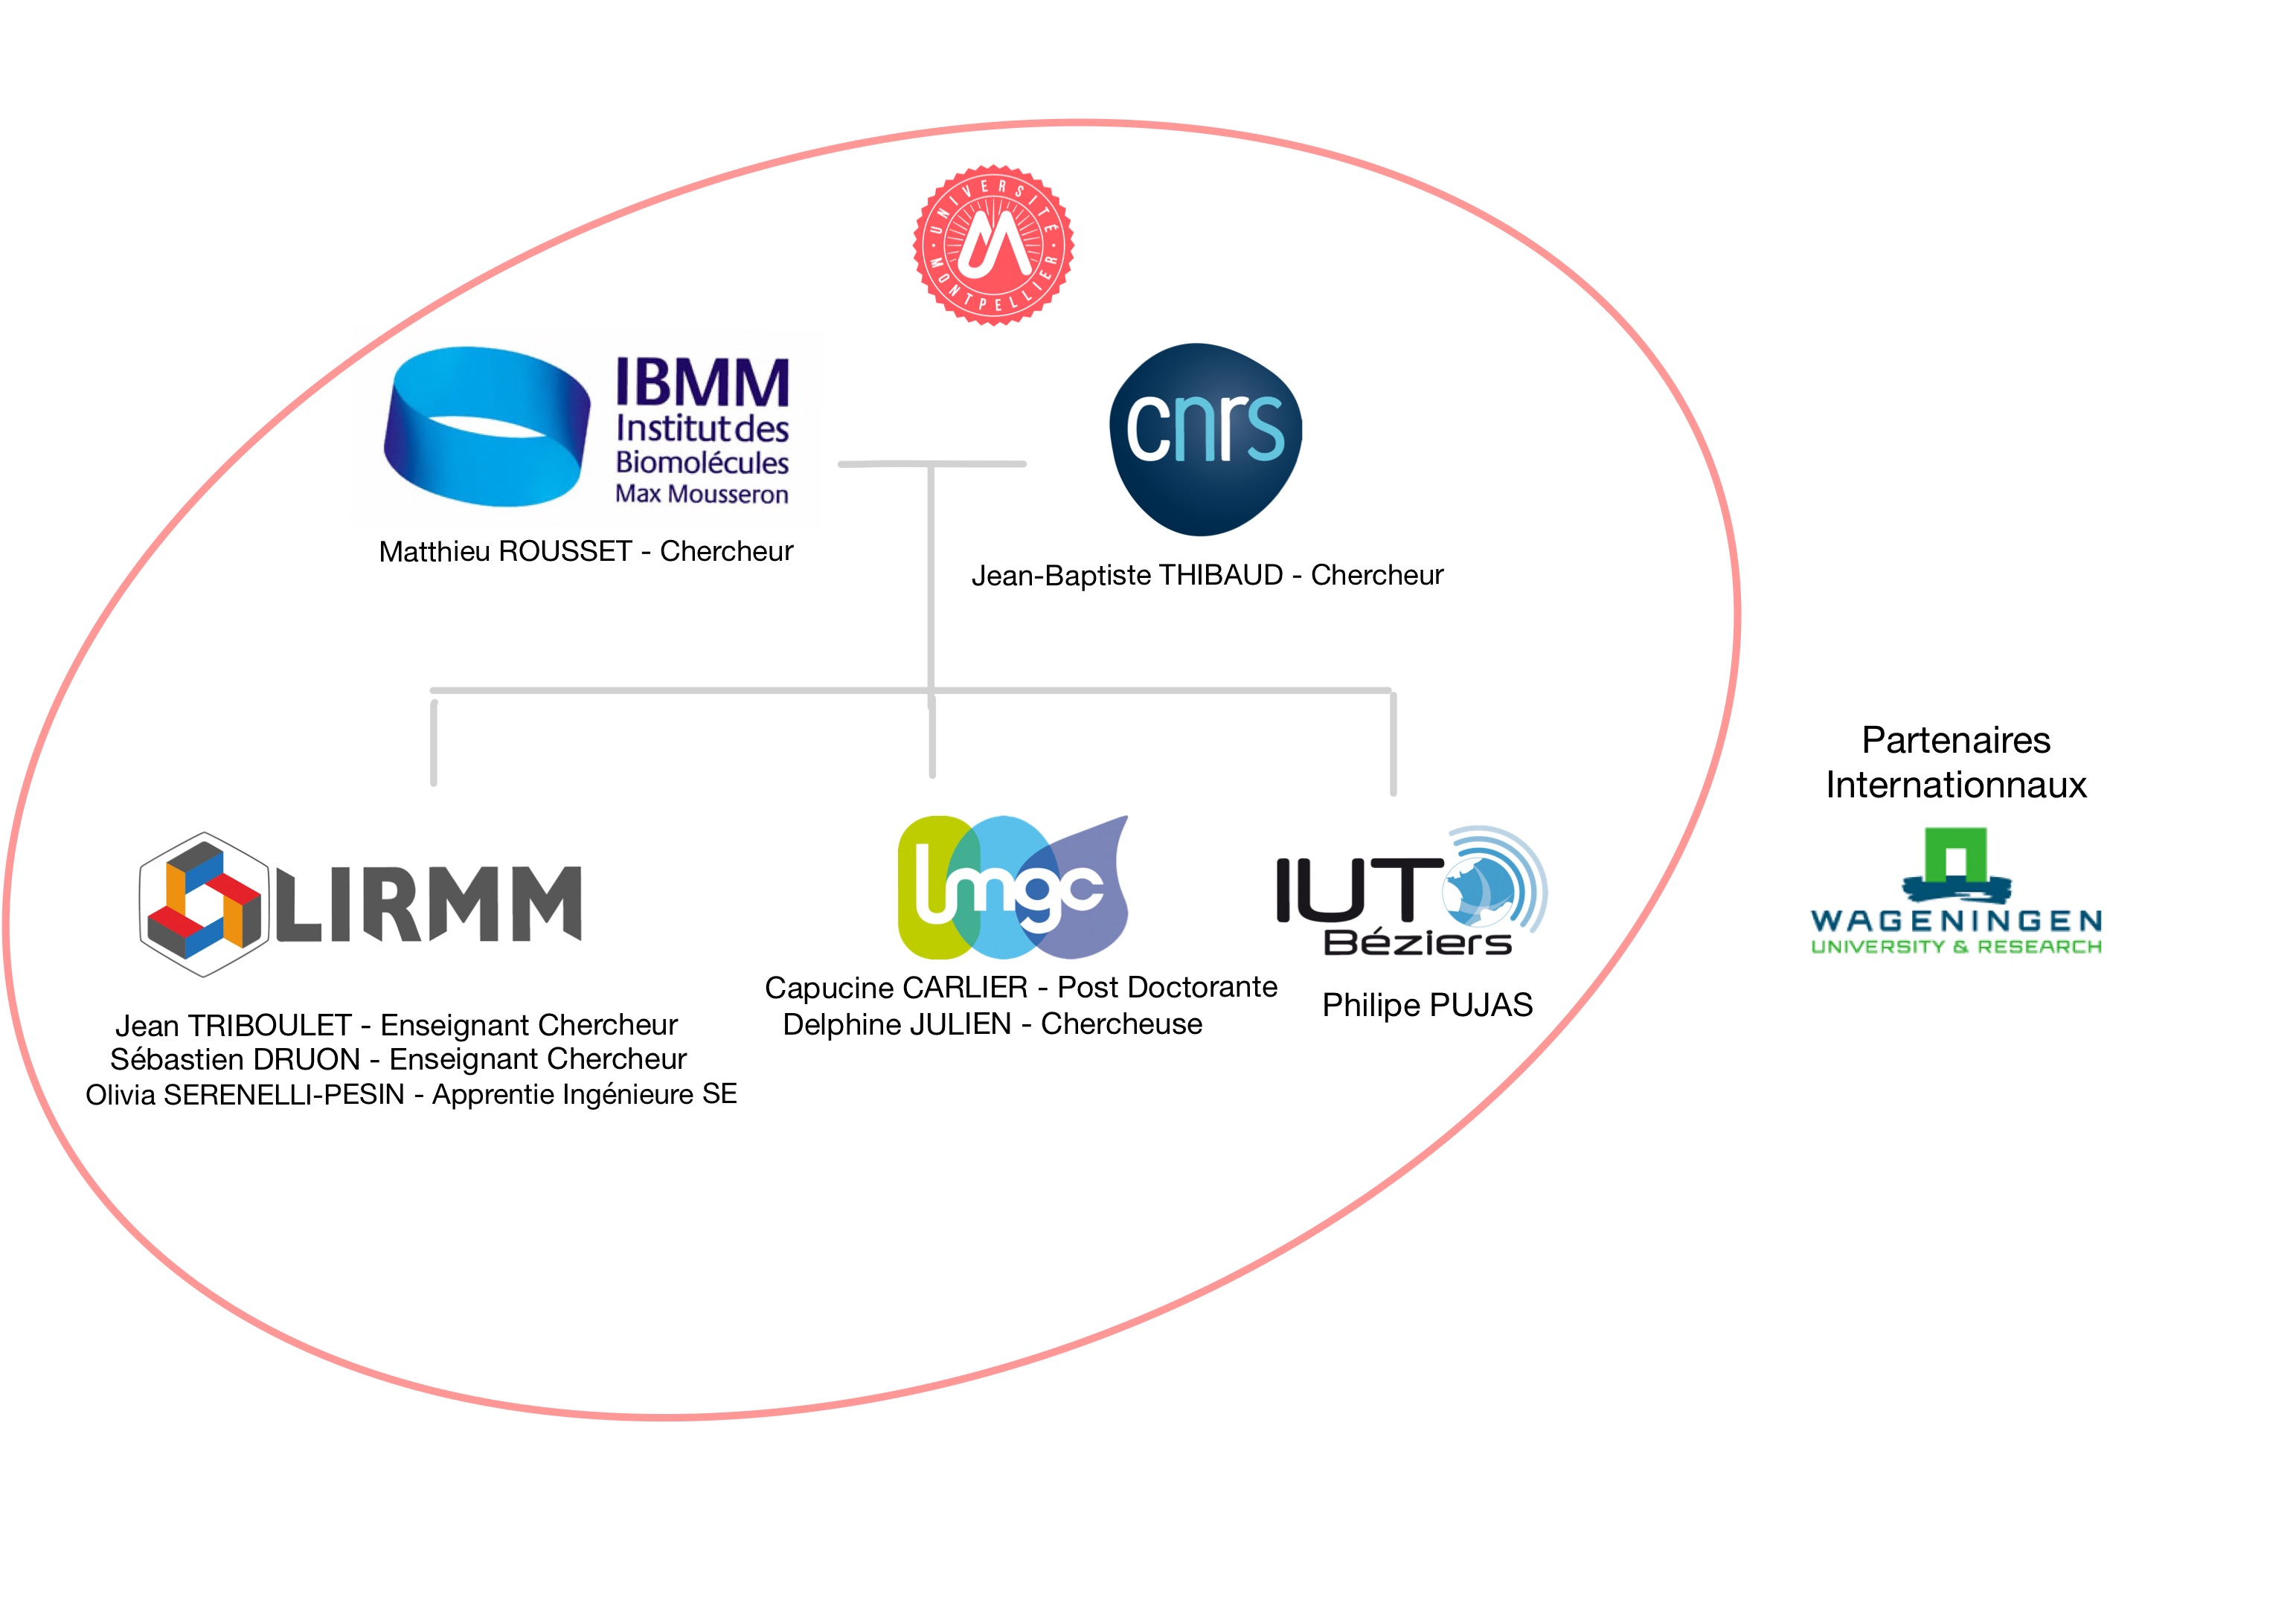
\includegraphics[width=15cm]{./img/orga.jpg}
    \caption{Organigramme de l'équipe}
    \label{orga_sbl}
\end{figure}

Au cours de mes missions, j'ai été et serai amenée à rencontrer tous les participants du projet, le plus souvent des biologistes.
Le LIRMMM executant les parties techniques (gestion du réseau et des données), le traitement des images et des algorithmes de reconnaissances, 
nous devons questionner les biologistes  sur les contraintes autours des abeilles et de leur environnement afin d'adapter la ruche plate et mettre 
en place les meilleures installation pour nos mesures. 


\subsection{Les missions autours de la ruche}
La ruche SuperBeeLive est composée de beaucoup d'élements différents, nécessitants tous des compétences diverses.
\begin{figure}[!h]
    \centering 
    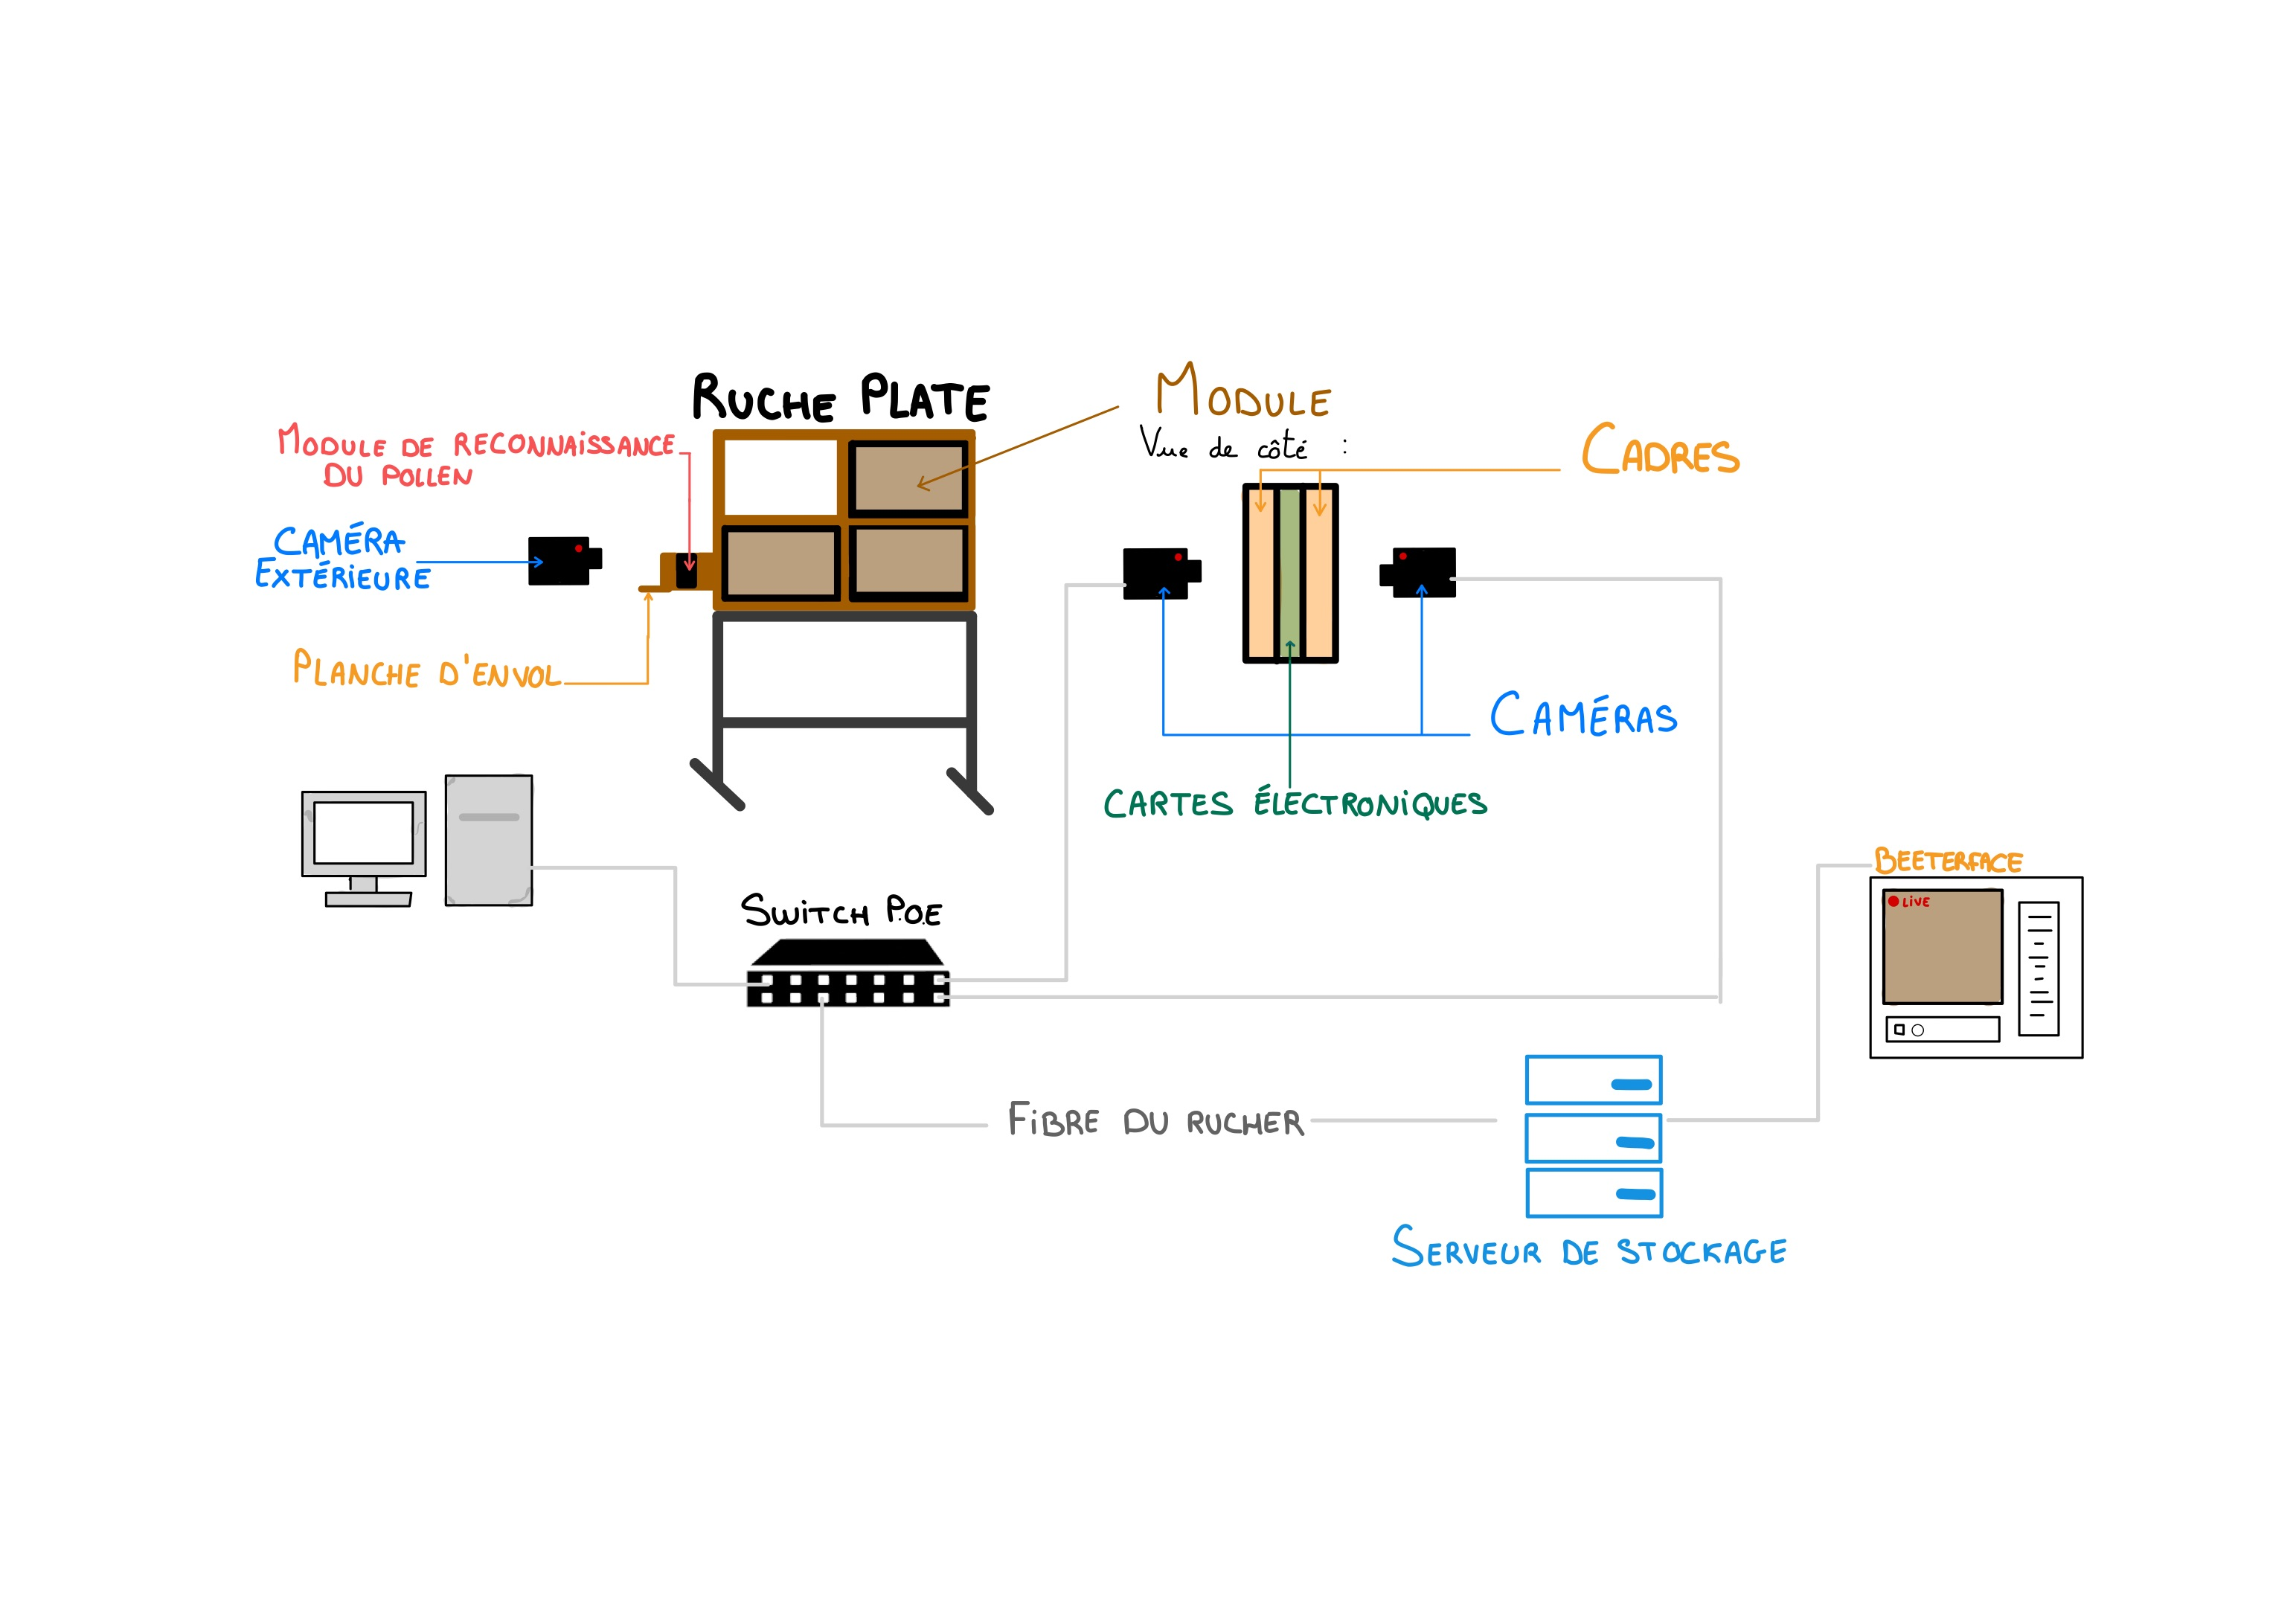
\includegraphics[width=20cm]{./img/resume_hive.jpg}
    \caption{Schéma récapitulatif de la ruche SuperBeeLive}
    \label{resume_hive}
\end{figure}
Sur le schéma \footnote{Voir figure \ref{resume_hive}}, nous pouvons voir un récapitulatif composantes de la ruche plate. 
Notre prototype se base sur un modèle à quatres Module. Chaque module est recto-verso, avec des deux côté des cadres, 
qui constituent l'endroit où les abeilles vivent et se développent. Entre elles, un espaces pour y glisser une carte électronique 
que je vais devoir confectionner afin d'avoir les capteurs nécessaires pour faire la remontée des données. 
Des deux côtés de chaques modules se trouvent des caméras. Celles-ci sont en noir et blanc et en haute résolution et ce sont elles
qui pourront nous fournir les images de l'intérieur de la ruche. Dans un premier temps, ces images seront remontées afin 
que les biologistes les annotent en fonction du comportement des abeilles. Avec ces annotations, l'équipe du LIRMM pourra s'occuper 
de créer les algorithmes de reconnaissances automatique. En plus de ces caméras qui permettent de voir l'intérieur de la ruche, une caméra à 
l'extérieur est également disposée. Celle-ci aura comme fonction de surveiller l'environnement extérieur et les possibles dangers comme
les frelons asiatiques. Toutes ses caméras sont reliée à un Switch Power Over Ethernet, c'est à dire qu'il permet de les connecter au réseau
du rucher, mais aussi de les alimenter. Un module de reconnaissance du pollen est mit en place à l'entrée de la ruche. Il a pour but 
de reconnaître les types de pollens que rapportent les abeilles. Tout comme la ruche, il est à l'état de prototypes et sa réalisation 
est assurée par un membre de l'Institut d'Electronique et des Systèmes (IES). 

Une fois les informations récoltées par les caméras, les cartes électroniques et le module de reconnaissance, elles sont envoyées 
sur le serveur de stockage du projet grace à la connection fibrée fournie par le CNRS. Une fois stockée, nous pourrons accéder à ces 
vidéos via l'application beeterface qui permet d'annoter les vidéos et de les visionner. 

Ce prototype contiendra tous les modules imaginés à ce jour pour récolter un maximum d'information sur les abeilles. Une fois
cette récolte de données précise réalisée, nous pourrons utiliser ces ressources afin de rendre la reconnaissance de comportement 
et d'événement automatique. 


\section{Mes lieux de travail}

Je travaille principalement au bâtiment 5 du LIRMM au campus Saint Priest de Montpellier où se trouve mon bureau. 
Je me rend également jusqu'à deux fois par semaine à l'IUT de Béziers\footnote{Voir figure \ref{lirmm_iut}} où se trouve une antenne du laboratoire afin de suivre
mon maître d'aprentissage lorsqu'il y a cours, mais aussi pour pouvoir remplir certaines de mes missions, comme l'encadrement
technique des projets étudiants. 

Enfin, afin de tester nos installations au fur et à mesure, un prototype de la ruche plate est installée au rucher du CNRS
\footnote{Voir figure \ref{rucher_exp}}.

\begin{figure}[!h]
    \centering 
    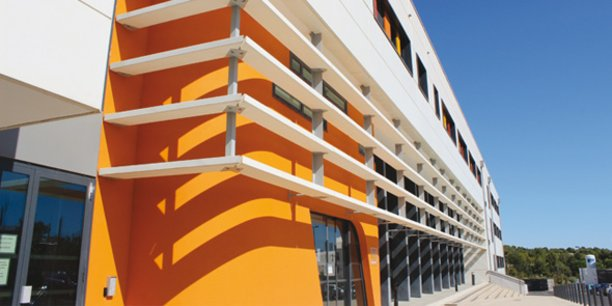
\includegraphics[width=7cm]{./img/photo_lirmm.jpg} 
    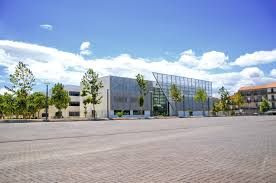
\includegraphics[width=7cm]{./img/iut_beziers.jpeg} \\
    \caption{Mes lieux de travail principaux le LIRMM et l'IUT de Béziers}
    \label{lirmm_iut}
\end{figure}

\begin{figure}[!h]
    \centering 
    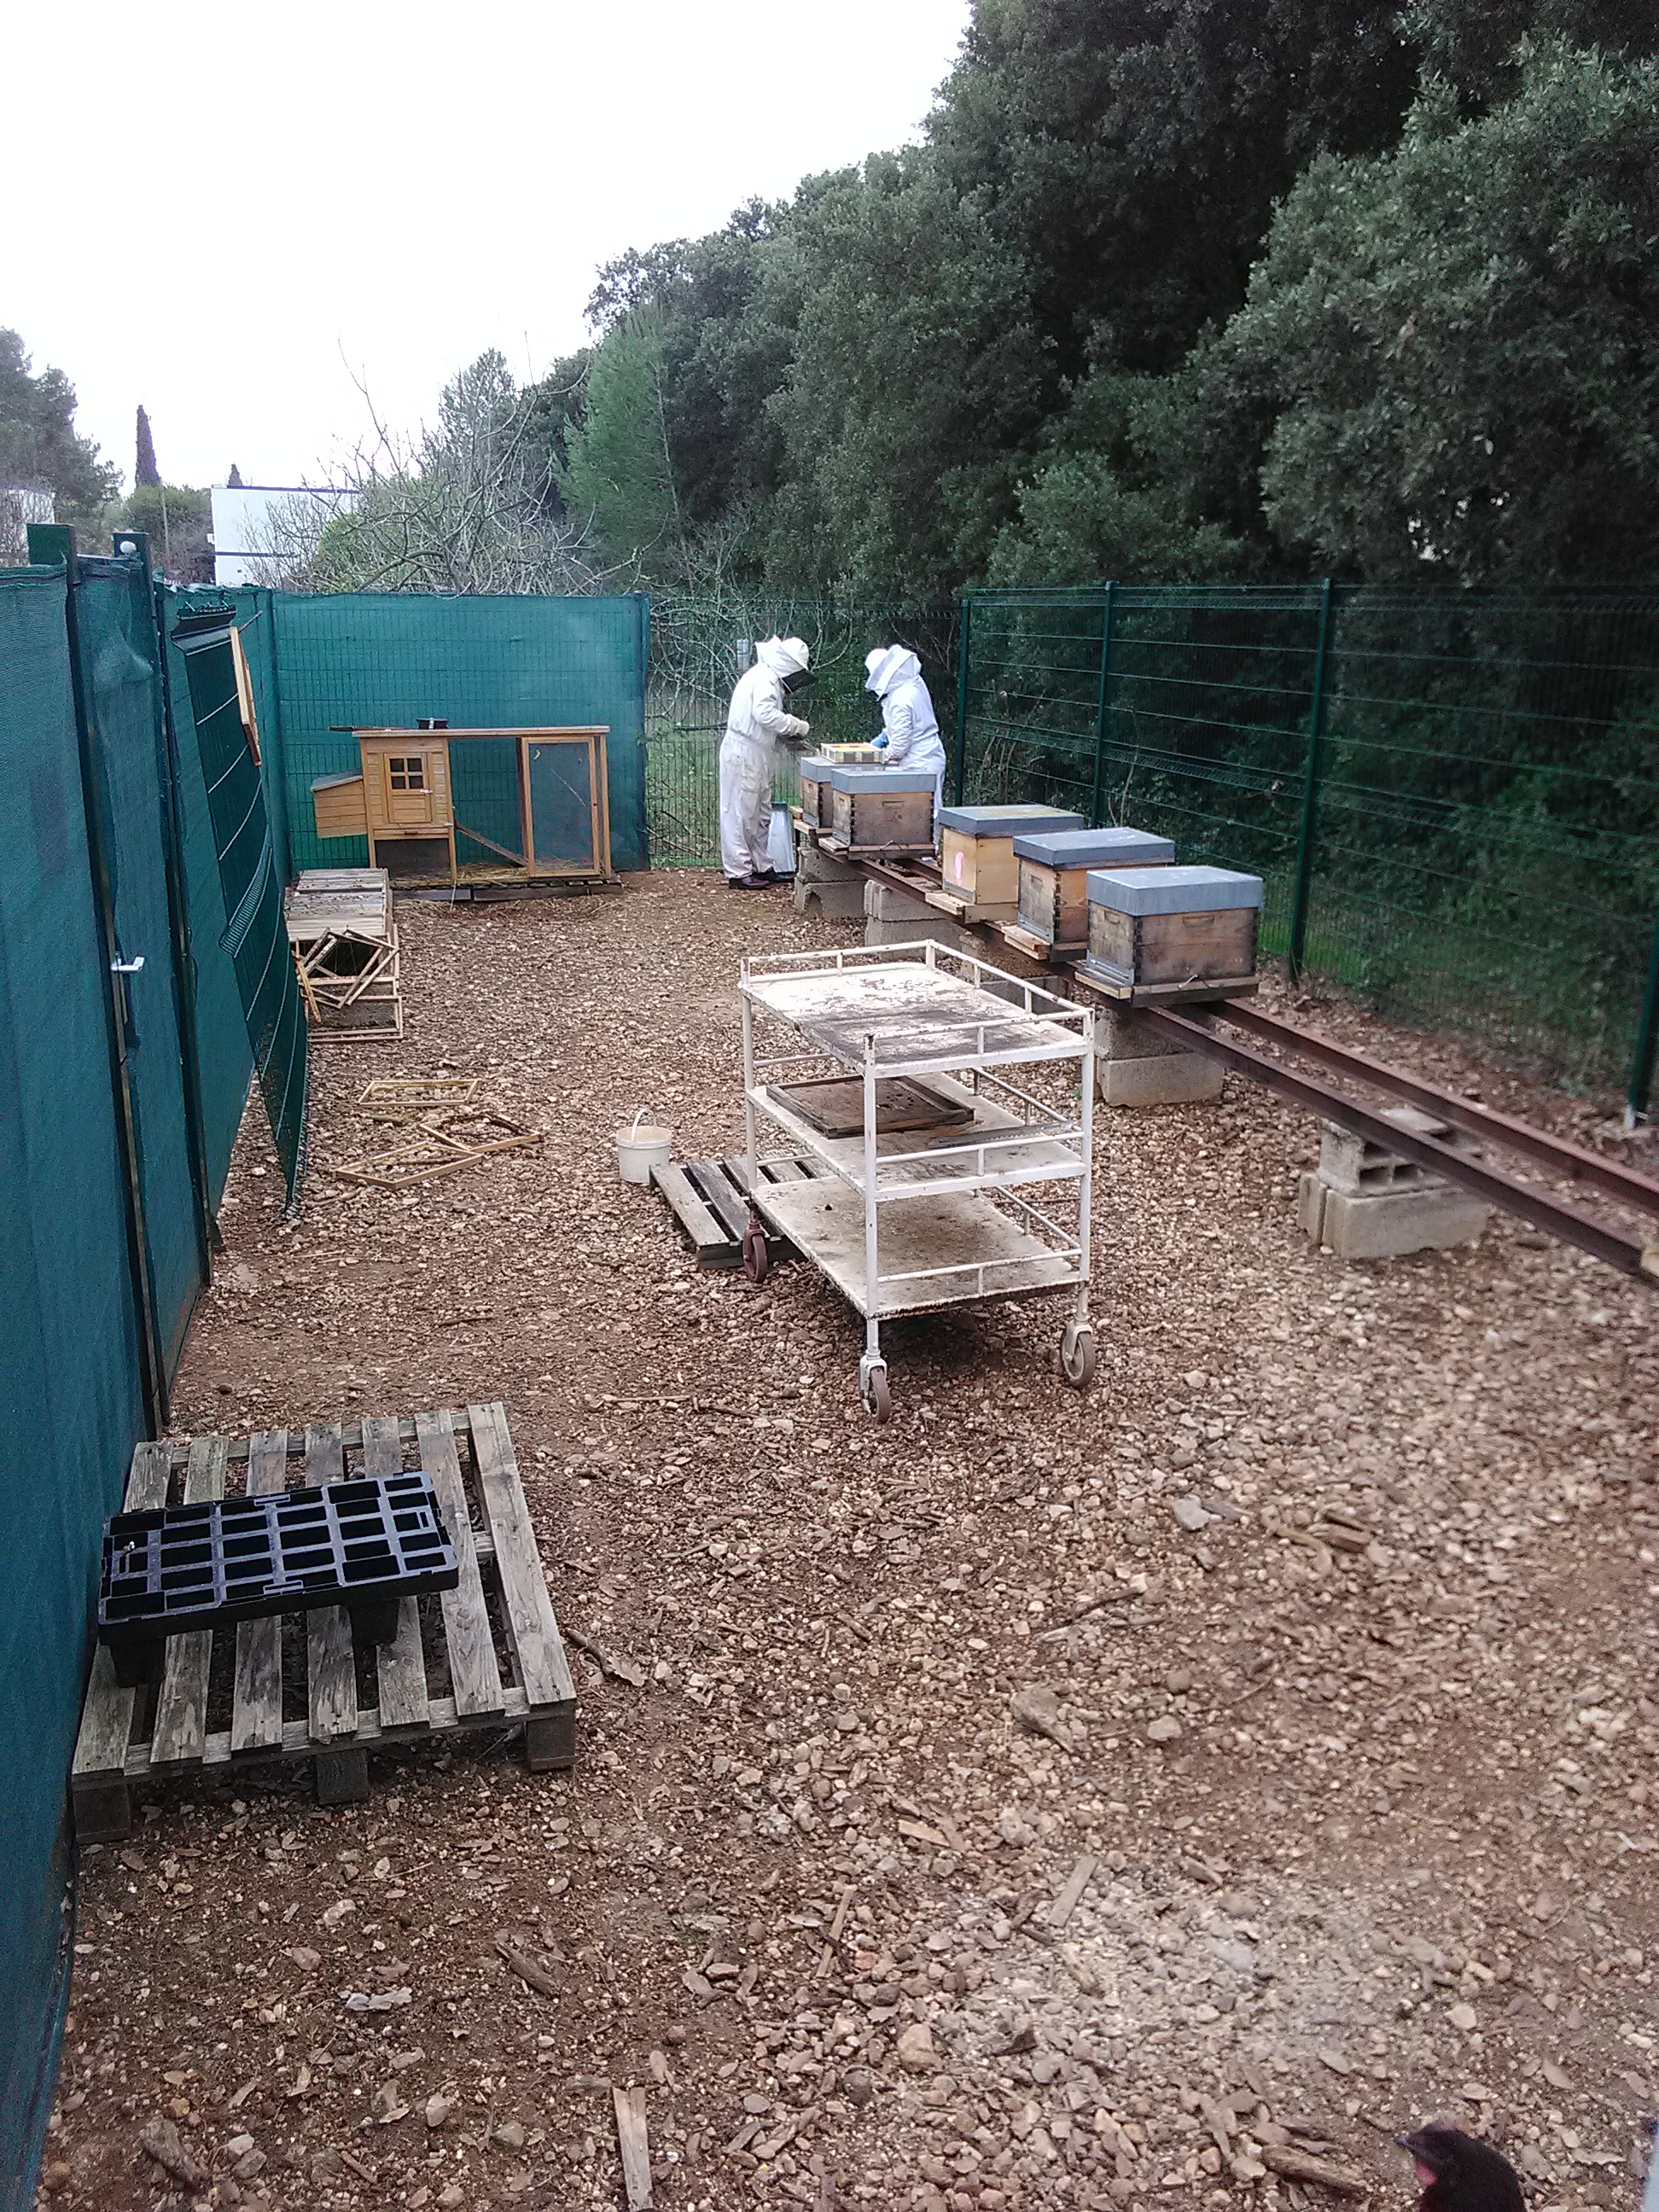
\includegraphics[width=5cm]{./img/photo_ext_ruche.jpg} 
    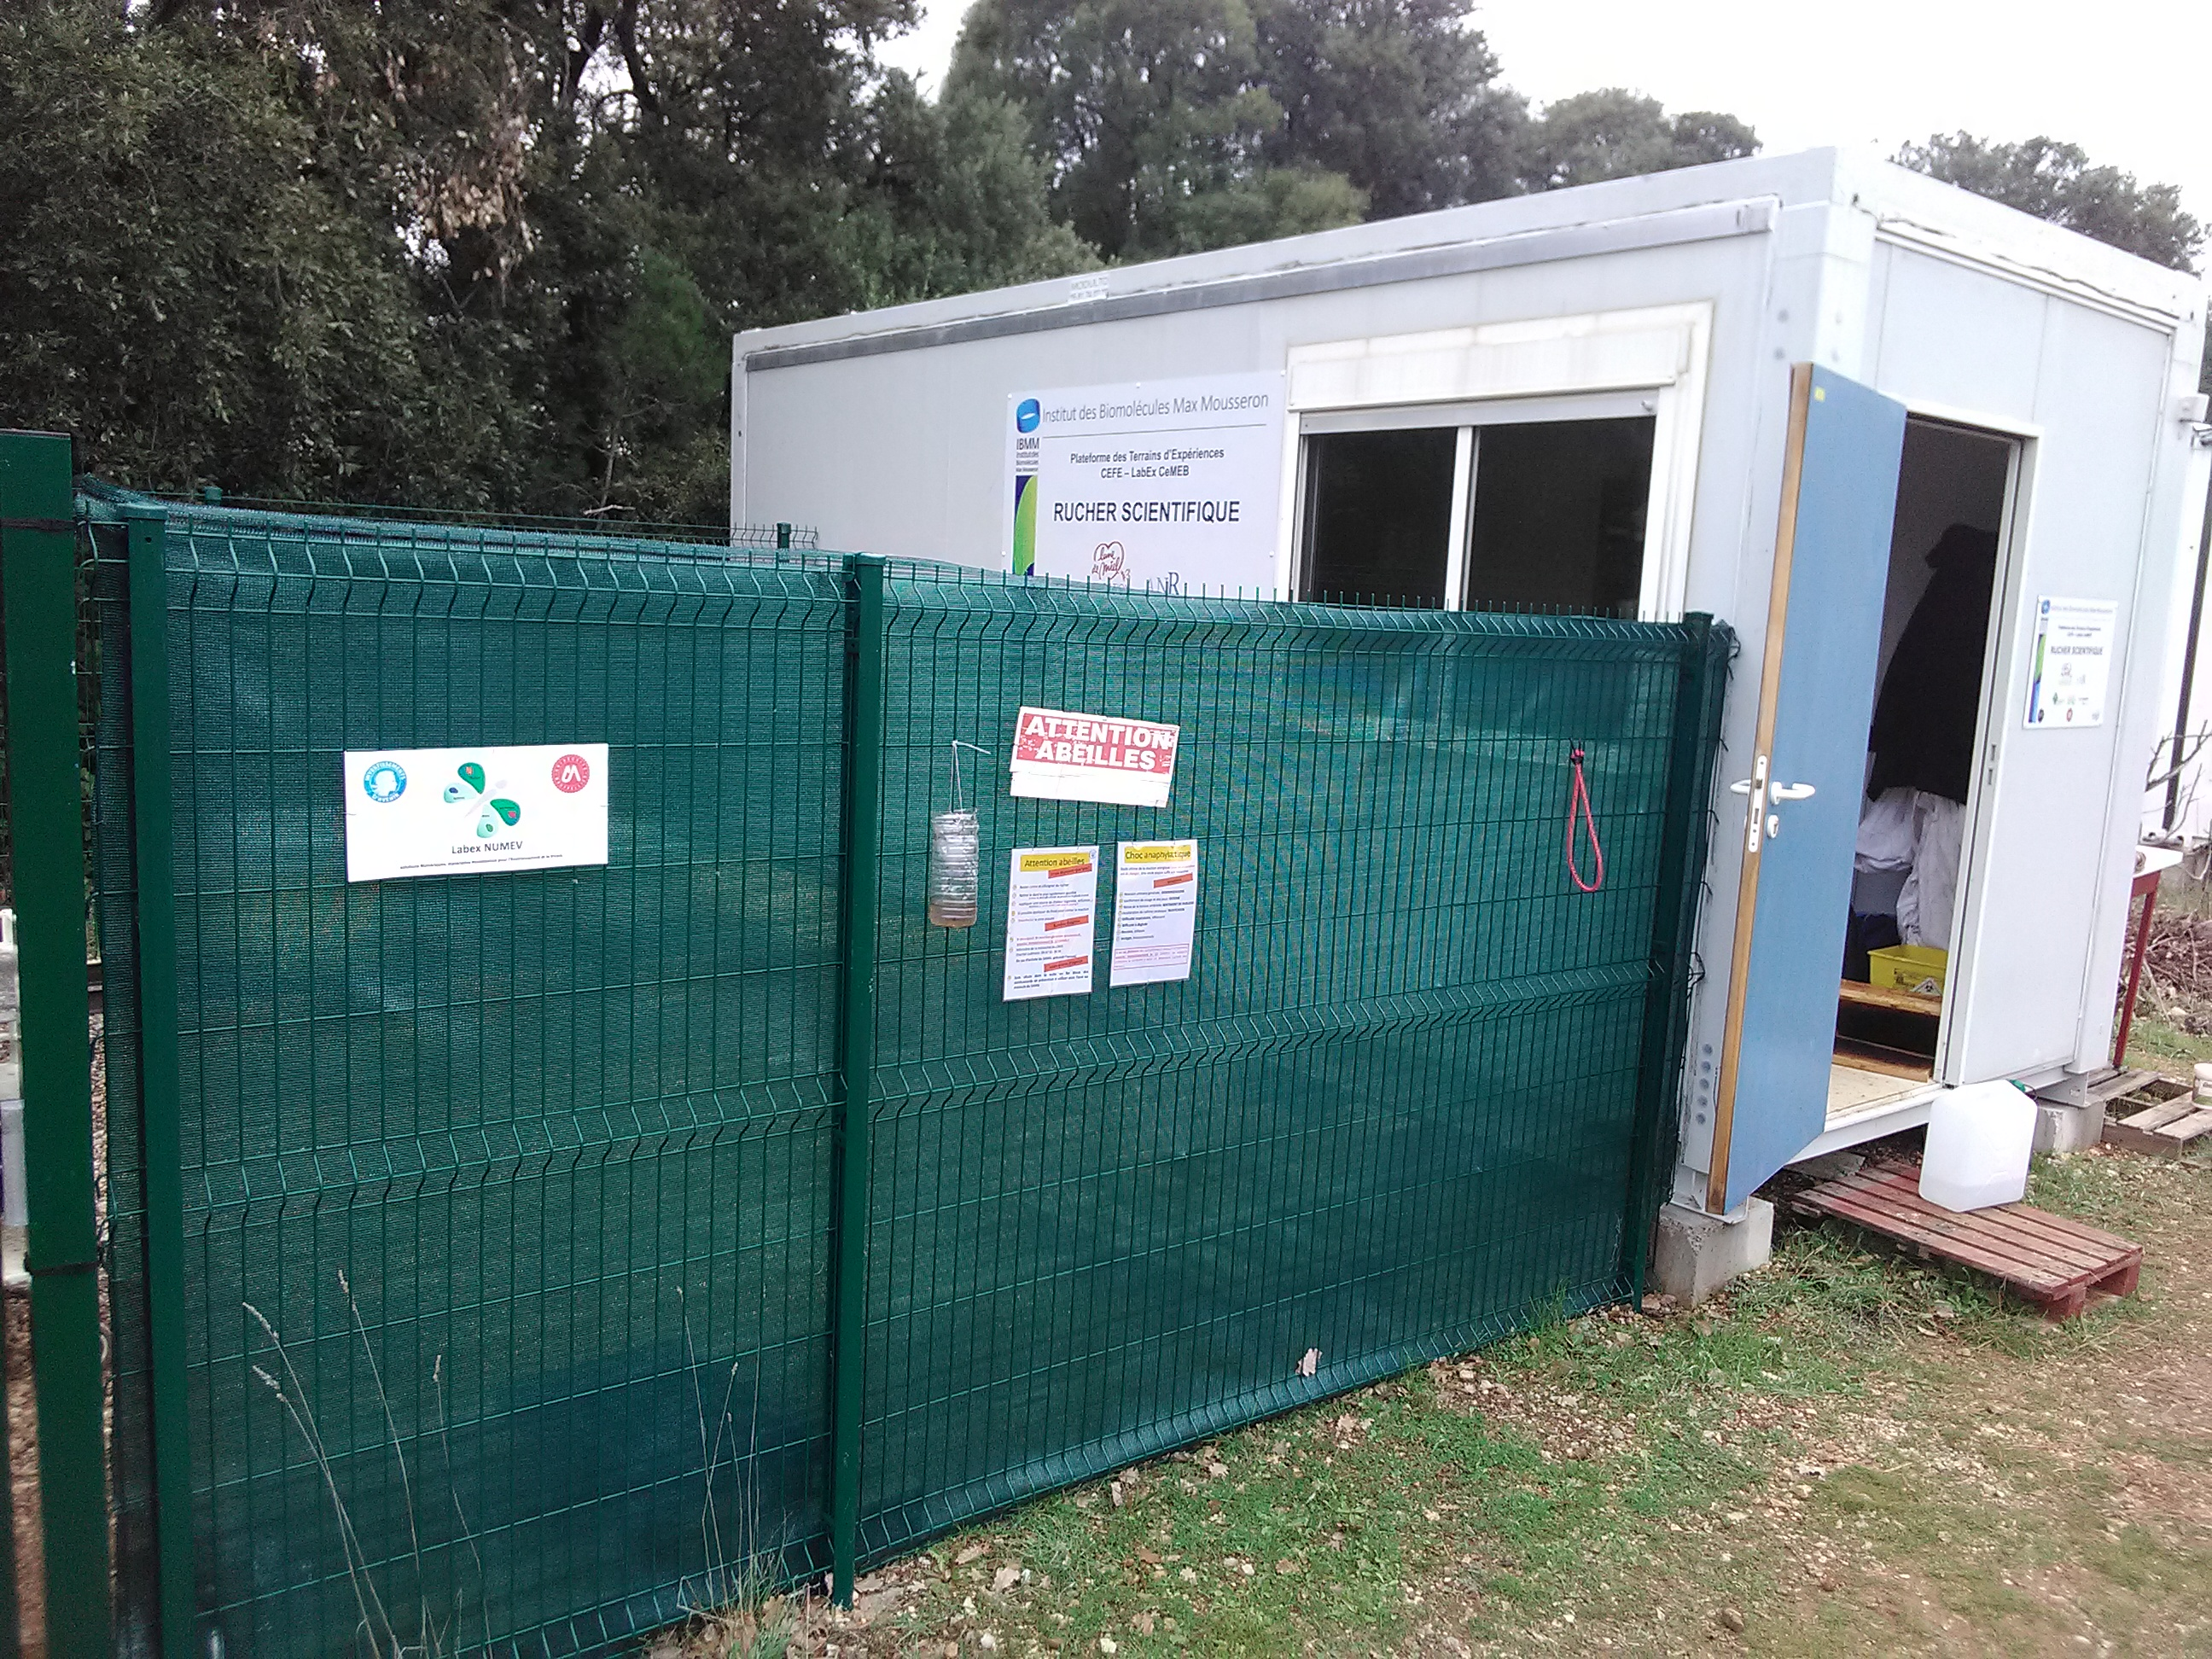
\includegraphics[width=5cm]{./img/photo_ext_prefab.jpg}
    \caption{Le rucher expérimental du CNRS}
    \label{rucher_exp}
\end{figure}


\chapter{Mes missions}
Au vu du nombre de tâches diverses à réaliser et de la taille de l'équipe, il est attendu que nous soyons multitâche. Tout 
au long de mon apprentissage, il me sera confié plusieurs types de tâches, allant de la conception à la réalisation de la 
carte électronique, à sa programmation. En terme de technique, la gestion du réseau du rucher fera également partie de mes missions.
Sur un autre plan, des tâches de gestion humaine me seront confiées via l'encadrement de stagiaire de Master, 
mais aussi via un travail de consultant technique pour les projets de premier années de DUT Réseau et Télécommunication. 

Ainsi, nous travaillons principalement à deux sur toutes les parties du projet SuperBeeLive, mon maître d'apprentissage me
confiant la gestion de nos parties du projet SuperBeeLive. 

\section{Formation préliminaire}
Afin de pouvoir m'intégrer dans le framework technique de mon équipe, il a été nécessaire
que je me forme à plusieurs outils. Tout d'abord, nous utilisons principalement le langage C pour la programmation.
De plus, pour travailler à plusieurs sur les codes, nous utilisons git et github. Pour ce qui est des écrits professionels, 
il m'a été vivement conseillé d'utiliser LaTeX. Enfin, pour utiliser ces outils, je me suis aussi formée à l'éditeur 
de texte VIM. 
Pour me former à ces outils, j'ai lu quelques livres et sites qui m'ont été également conseillés par mon maître d'apprentissage
\footnote{Voir bibliographie : \cite{ref4}, \cite{ref5}, \cite{ref6}, \cite{ref7}, \cite{ref8}, \cite{ref9}}

\section{Missions principales}
Il a été décidé de séparer mes missions en deux grandes catégories : principales et annexes. Ainsi, mes missions principales 
seront celles qui auront toujours la priorité sur les annexes. Elles concernent les parties les plus techniques 
et liées directement à mon domaine d'étude. Seulement, avant même de commencer ces missions, j'ai dû m'autoformer sur 
quelques outils afin de pouvoir travailler avec mon maître d'apprentissage. 

\subsection{Création de la carte électronique}
La tâche principale de ma première année d'apprentissage est la création des cartes électroniques qui seront inserées dans 
les cadres du rucher. 
Notre but est de pouvoir récolter plusieurs types d'informations afin de les reporter le plus précisement possible sur une carte 
représentant le cadre et les valeurs récoltées. 
Ainsi, les biologistes pourront mettre en liens des informations telles que la températures ou l'hygrométrie avec les images 
prises par les caméras. 
Afin de réaliser cette carte, deux grandes étapes sont nécessaires : la maîtrise du microcontrôleur qui sera installé sur la 
carte avec les capteurs, et le dimensionnement de la carte avec le choix des capteurs. Une fois ces deux étapes faites, nous pourrons 
passer à la réalisation d'un premier prototype, idéalement pour l'été prochain. 

Le microcontrôleur que je vais devoir utiliser pour le contrôle de la carte est le STM32. Ce choix a été fait par M. Druon. 
Ainsi, il m'est demandé de connaître au mieux ce Microcontrôleur afin que lorsque nous serons amenés à le programmer et à l'utiliser, 
je sois la référence de l'équipe en ce qui le concerne. 
Pour cela j'ai, entre autre, plusieurs livres le concernant \footnote{Voir \cite{book1}}. 
De plus, nous désirons ne pas dépendre d'un IDE pour le développement avec la STM32. Il m'a été demandé de mettre en place 
une toolchain (chaine de compilation) pour Ubuntu et STM32 avec un guide d'utilisation. 
Avec ces outils, nous aurons une base solide pour travailler avec ce microcontroleur. 

Une fois ce premier travail réalisé, l'équipe sera opérationnelle pour le dimensionnement de la carte. Cette partie du travail
commencera par une étude des besoins et des ressources à disposition afin de choisir les capteurs en fonctions ce que nous pouvons
et devons faire. 
Les contraintes venant en grande partie de la place réservée pour les cartes électroniques dans les prototypes du rucher, mais 
aussi des conditions qu'imposent un tel milieu (activité des abeilles, température...). 
Plusieurs étapes viendront consituer ce dimensionnement, comme des tests avec un petit nombre de capteurs avant de concevoir la
première carte électronique. 

\subsection{Développement d'un logiciel d'annotation pour les biologistes}
L'une des finalités du projet SuperBeeLive est d'avoir un ou plusieurs algorithmes capables de reconnaître automatiquement 
des comportements des abeilles, comme leur dances, des regroupements, ou des messages qu'elles se transmettent de diverses manières.
Ainsi, afin de pouvoir alimenter les bases de données permettant d'arriver à de tels algorithmes, il est nécessaire d'avoir 
déjà des vidéos annotées avec les informations permettant de repérer les dits comportements. 
Afin de faciliter cette tâche, qui sera surtout réalisée par les biologistes, ma première mission dans leur équipe lors de mon 
stage de fin de DUT avait été de développer un logiciel d'annotation vidéo. Ce logiciel, correspondant aux besoins exacts des 
biologiste, permettra, une fois fini, d'annoter avec des figures disposables sur les vidéos, des textes et des tags permettant de
classer et retrouver les vidéos facilement, d'avoir une base de donnée précise et utilisable pour que les roboticiens (LIRMM) puissent
l'exploiter. 

\begin{figure}[h!]
    \centering
    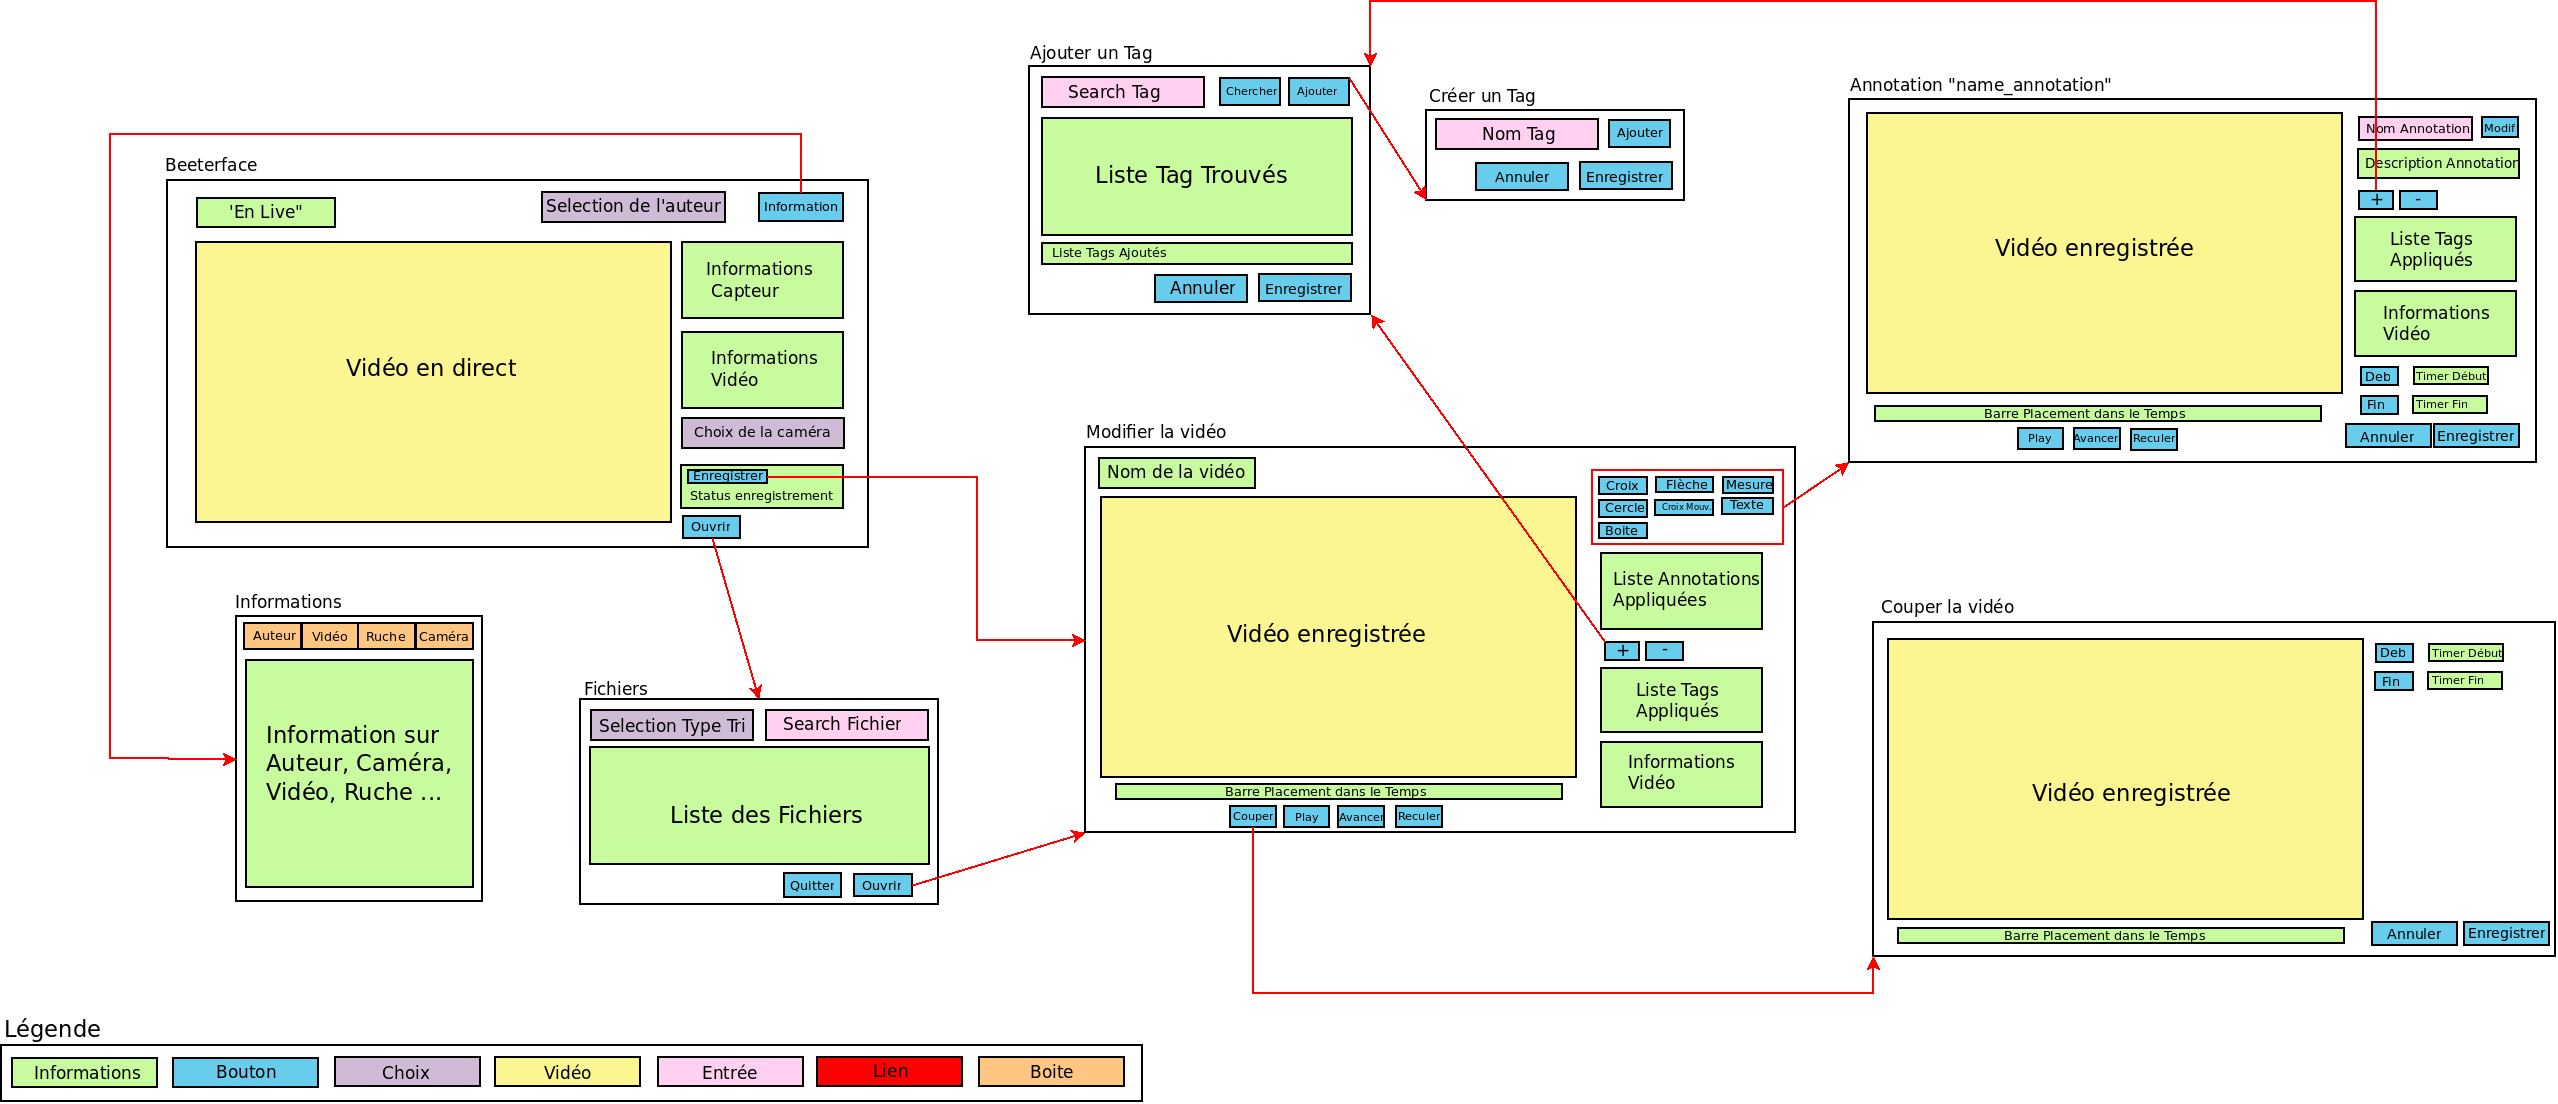
\includegraphics[width=17cm]{./img/schema_interface.png}
    \caption{Synoptique de l'interface}
    \label{syn}
\end{figure} 

Aujourd'hui, toute la partie graphique a été réalisée, et nous avons déjà une interface bien 
définie \footnote{Voir la figure \ref{syn}}
Il reste encore du travail concernant le lien entre les capteurs, les caméras etc et l'interface ainsi que la sauvegarde
des données sur nos serveurs. 

Le développement de ce logiciel, même si bien avancé, n'est pas encore fini et a pour projet de l'être d'ici la fin de l'année 2020. 
J'ai donc comme mission de finir son développement avec mon maître d'apprentissage et surtout de le mettre à jour en corrigeant les 
possibles bugs et en prenant en compte les retours utilisateurs lorsque celui-ci sera disponible. 


\section{Missions annexes}
\subsection{Mise en place et gestion du réseau du rucher et de ces équipements}
Nous travaillons sur une ruche plate expérimentale, celle-ci est installée au CNRS et il a été tiré deux fibre afin d'avoir 
une connexion internet rapide et assez conséquente par rapport aux données qui sont prévues d'être enregistrées et envoyées. 
En effet, les biologistes ont exprimé le besoin de sauvegarder la casi intégralités des vidéos et données numériques des capteurs
de la naissance à la mort de la ruche, ce qui serait une première en terme de données autours des abeilles. Seulement, 
une telle sauvegarde de données nécessite un réseau solide sur place mais aussi et surtout un serveur avec une capacité 
de stockage assez conséquente afin de pouvoir supporter un tel flot de donnée (de l'ordre du petaoctet). 
Le dimensionnement du serveur a été fait et sera confirmé par l'équipe informatique du LIRMM, mais une connaissance 
de l'architecture et de la configuration du serveur dans l'équipe directement est primmordiale pour pouvoir travailler dessus
et gérer directement la sauvegarde des données. 
Il m'a donc été demandé de suivre cette installation et d'avoir une veille technologique concernant le serveur et l'architecture
utilisées. 

Enfin, quelques équipements réseau ont été et vont être installés au rucher \foonote{Voir figure \ref{}}. 
Leur mise en place et gestion m'ont également été confiés.

\begin{figure}
    \centering
    \includegraphics[scale=0.7]{}
    \caption{Réseau du rucher}
    \label{reseau_rucher}
\end{figure} 


\subsection{Gestion de projets étudiants}
Afin de me familiariser avec l'encadrement, travail majeur en tant qu'ingénieur, il m'a été confié le suivi technique de six projets IoT 
à des étudiants de première années de DUT Réseaux et Télécommunication. Ainsi, je suis ces différents groupes à travers des rapports 
d'avancement qu'ils m'envoient régulièrement et je leur fais des retours par mail ou par rendez-vous à l'IUT de Béziers. \\
Ce travail me permet de mettre en place une organisation dans mon travail par rapport à mes obligations les concernants, mais aussi
de voir d'un oeil extérieur comment ils organisent leur projet et de les conseiller un maximum. 
L'idée avec ce premier encadrement est de me confier un stagiaire de 1ère année de Master l'année prochaine, afin que je l'encadre de A à Z 
sur une mission en lien avec le projet SuperBeeLive. 


\section{Missions à venir}
Les prochaines missions qui me seront confiées auront pour but de m'intégrer de plus en plus dans les différentes composantes du projet
SuperBeeLive. J'aurai à renforcer mes connaissances en VHDL mais aussi en traitement de données images et vidéos afin de participer à 
la partie reconnaissance du comportement des abeilles plus activement. 

\chapter{Le rapport au DDRS de l'entreprise}
Aujourd'hui, les enjeux autours du Développement Durable prennent une place
de plus en plus importante dans un contexte socio-économique où la santé de notre
planète est en jeux. Le défis est de réussir à continuer les avancées et développement, 
notament en matière de technologie. En ce sens, la recherche est un milieu qui doit être 
particulièrement attentif à ces questions : les nouvelles idées et leurs applications ne 
peuvent pas se permettre d'être contraire aux enjeux de notre siècle.
Ainsi, en recherche nous retrouvons de plus en plus de sujets visant à améliorer notre impact 
écologique et à mieux connaîre nos impacts et les dangers qui entourent la nature. 
C'est d'ailleurs le cas du projet SuperBeeLive qui, une fois à terme, permettra de connaître 
bien plus les abeilles et leur environnement afin de sensibiliser et mettre en place des solutions afin de les 
protéger.

Dans ce contexte où la recherche a un fort impact direct sur le développement durable, on pourrait 
s'attendre à des mesures concretes de la part des laboratoires de recherches. Seulement, dans le dernier
rapport d'évaluation du LIRMM, datant de janvier 2019, il est indiqué que :
"citation" 


Le LIRMM n'a pas de charte de développement durable, ni de section consacré à ces enjeux dans le réglement intérieur du site. Cependant, 
les achats fait par le LIRMM visent à limiter leur impact écologique. Par exemple, une rationalisation des impressions est mise en place. 
De plus, au niveau de la flotte de véhicule du LIRMM, l'achat d'un véhicule utilitaire a été mutualisé avec les autres laboratoires du campus 
saint priest. Par ailleurs, le second véhicule du laboratoire étant en fin de vie, il est prévu de le remplacer par un véhicule électrique, 
un choix qui coûte plus cher mais qui est préféré pour limiter l'impact environnemental.

D'un point de vu plus large, nous pouvons regarder ce qui est mis en place au niveau de l'Université de Montpellier. 
Au quotidien, nous pouvons remarquer qu'une certaine attention est apportée aux enjeux DDRS. 
Tout d'abord, la grande majorité des véhicules utilisés pour les déplacements dans et entre les différents lieux qui constituent l'UM sont
électriques. Ensuite, les machines à café qui ont été installées en remplacement des ancienne ont des gobelets en cartons pour les 
grandes boissons, et les touillettes on étés récemment remplacées par des touillettes en bois dans la majorité des établissements. 
Toujours en lien avec le café, notons qu'il est fortement encouragé d'utiliser une tasse personnelle pour se servir des machines à café : 
dans les laboratoire surtout, presque tous les employés ont leur propre tasse réutilisable. 
Ensuite, il est important de noter que des poubelles avec plusieurs sacs pour trier les déchets sont installées dans tous les établissements 
égalements : il est rare de trouver des poubelles avec un unique sac. Notons que dans les bureaux et salles de cours, nous retrouvons des poubelles 
avec un compartiment pour le papier. 

Enfin, nous pouvons aussi soulever le fait que l'école Polytech est très engagées dans la politique de DDRS : elle met en place des 
actions pour limiter leur impact environnemental et informe les étudiants, futurs ingénieurs, afin qu'ils soient 
conscient des enjeux auxquels nous allons faire face dans notre métier. Ces informations sont faites via des cours, mais aussi 
des conférences proposées gratuitement et accessibles à tous, comme par exemple celle donnée le 24 février 2020 par Jean-Marc JANCOVICI 
"Générations Futures" qui nous a présentés le paysage global des enjeux climatiques, leurs conséquences et leurs causes. 
L'école Polytech peut être considéré comme le porte étandard de l'Université de Montpellier concernant le Développement Durable à ce jour. 
Il est alors important de suivre ce mouvement et d'encourager l'UM de faire plus concernant le DDRS. 


\chapter{Conclusion}
Être dans un laboratoire de recherche pour l'apprentissage du métier d'ingénieure en électronique n'est pas commun. Les enjeux et responsabilités 
qui me sont confiées ne sont pas du même ordre que si j'avais été dans une entreprise privée. Seulement, c'est un aspect du métier qui est tout aussi
intéressant : la pluridisciplinalité et le besoin d'apprentissage constant sont deux composantes du milieux très intéressantes à travailler. 
D'un point de vue technique, je serai amenée à mettre en pratique une grande partie des compétences vues en cours, puisque nous nous occupons de 
la réalisation de la plupart des parties de la ruche SuperBeeLive de A à Z. 
Les responsabilités qui me sont données concernant le projet SuperBeeLive et l'encadrement d'étudiant me permettent d'intégrer petit à petit le rôle de 
l'ingénieur dans une équipe, allant de la gestion du temps, du matériel, de l'argent à la gestion humaine. 

Cet apprentissage va me permettre d'intégrer petit à petit le monde de la recherche, me permettant de comprendre les enjeux, la façon de travailler, 
et le fonctionnement de ce milieu. 


\bibliographystyle{plain}
\bibliography{biblio}


\end{document}  
